% !TEX encoding = UTF-8
\documentclass[a4paper]{report}
%Options: Sonny, Lenny, Glenn, Conny, Rejne, Bjarne, Bjornstrup
%Nice ones : Lenny, Glenn, Bjornstrup
\usepackage[Lenny]{fncychap}
\usepackage[utf8]{inputenc}
\usepackage[english]{babel}
\usepackage[T1]{fontenc}



%math 
\usepackage{amsmath} %Normal math
\usepackage{amssymb} %Math symbols
\usepackage{centernot}

%Algorithmic
\usepackage{algorithm}
\usepackage[noend]{algpseudocode}

%Chimie
%\usepackage[version=3]{mhchem}
%cf http://fr.wikibooks.org/wiki/LaTeX/%C3%89crire_des_formules_chimiques

% Allows for temporary adjustment of side margins
% Lorsque les tableaux sont trop grands
\usepackage{chngpage}

% provides filler text
\usepackage{lipsum}
% usage : \lipsum[1]

% just makes the table prettier (see \toprule, \bottomrule, etc. commands below)
%\usepackage{booktabs}

%Mise en page
\usepackage{graphicx}
\usepackage{caption}
\usepackage{subcaption}
\usepackage{fancyhdr}
\usepackage[top=3cm, bottom=3cm, left=4cm, right=3cm]{geometry}
\usepackage{listings}
\usepackage{xcolor}
%\usepackage{color}
%\usepackage{placeins}

%Frames/boxes
\usepackage{framed}


\definecolor{gris}{gray}{0.5}
\definecolor{code}{gray}{0.95}

% Table des matières cliquable 
\usepackage{hyperref}
\hypersetup{
    colorlinks, % empécher latex de colorer les liens
    citecolor=black,
    filecolor=black,
    linkcolor=black, % couleur des liens dans la table des matières
    urlcolor=blue
}

%Points dans la table des matières
\usepackage{tocloft}
\renewcommand{\cftsecleader}{\cftdotfill{\cftdotsep}} 
% Ligne de points dans la table des matières


%Adds bibliography to the ToC
\usepackage{tocbibind}
%notbib to remove the Bibliography notindex to remove the Index 
%nottoc to remove the Table of Contents 
%notlof to remove the List of Figures 
%notlot to remove the List of Tables - See more at: http://www.howtotex.com/packages/how-to-add-bibliography-and-more-to-table-of-contents/#sthash.gea9BJsw.dpuf

%Citation for bibliography. Use :
%\citet{KEY} --> Bester et al. (1998)
%\citep{KEY} --> (Bester et al. 1998)
\usepackage{natbib}


\DeclareGraphicsExtensions{.png}


\setcounter{secnumdepth}{3} %depth of numbering
%\setcounter{tocdepth}{3} %depth of table of content

%change item style
%\bullet (default), \circ  \triangleright, \divideontimes, \circledcirc  \bigstar \models \vdash \vDash \Vdash \circlearrowleft \circlearrowright \looparrowright (nice) \Psi \crux \heartsuit \clubsuit \spadesuit \surd \diamondsuit \blacktriangle \blacksquare \blacklozenge \blacktriangledown \sphericalangle \propto \maltese (nice) \checkmark
\def\labelitemi{$\looparrowright$} 
\def\labelitemii{$\propto$} 
%\def\labelitemiii{$\looparrowright$} 
%\def\labelitemiv{$\looparrowright$} 


%Page de garde

\newlength{\larg}
\setlength{\larg}{14.5cm}

% Pour corriger alignement, jouer avec la taille de tabular (± 6cm)
%%%PAGE DE TITRE%%%

\newcommand{\titleg}{
  \begin{titlepage}
  \begin{center}

  \bigskip
  \bigskip
  \bigskip
  \bigskip 
  \bigskip


  % Upper part of the page 
  \includegraphics[width=3cm]{./logo}\\[1cm]
	%\includegraphics[bb=0 0 30 30]{./logo}\\[1cm]
  \smallskip
  \textsc{\LARGE Université de Liège}\\
  \smallskip
  \textsc{Faculté des sciences appliquées}\\

  \bigskip


%1. thesis/dissertation director
%2. thesis/dissertation advisor
%3. thesis/dissertation committee chair

%Master thesis
  % Title 
  \rule{\columnwidth}{1pt} \\[0.4cm] 
  { \huge \bfseries Generic image classification : \\ \bigskip random and convolutional approaches}\\[0.4cm]
  \rule{\columnwidth}{1pt} \\[0.2cm]



  \begin{minipage}{0.7\textwidth} 
  \begin{center} \large 
  \textsc{Master thesis}
  \end{center} \end{minipage}

  \vfill
  %TODO image


  \begin{minipage}{0.7\textwidth} \begin{center}
  \textit{Thesis directors} \\
  \large Pierre \textsc{Geurts} \\
  \large Raphaël \textsc{Marée} 
  \end{center} \end{minipage} 

  \bigskip
  \bigskip
  \bigskip

  \textit{Author} \\
  \begin{minipage}{0.7\textwidth} \begin{center}
  \large Jean-Michel \textsc{Begon}
  \end{center} \end{minipage} 
  


  \bigskip
  \bigskip
  \bigskip

  \textsc{Année académique 2013-2014}
  \end{center}
  \end{titlepage}
}

%%%FIN PAGE DE TITRE%%%



\begin{document}

% Titre
\pagenumbering{Alph}
\titleg
\thispagestyle{empty}
\newpage
\pagenumbering{arabic}

% Mise en page
\pagestyle{fancy}
\lhead{}
\chead{}
%\lhead{\itshape \textcolor{gris}{\leftmark}} % display chapter name
\rhead{\itshape \textcolor{gris}{\rightmark}} % display section name
\lfoot{\itshape \textcolor{gris}{Generic image classification - The RandConv framework}}
\cfoot{}
\rfoot{\itshape \textcolor{gris}{\thepage}}
\renewcommand{\headrulewidth}{0.4pt}
\renewcommand{\footrulewidth}{0.4pt}

\newpage 


\tableofcontents

\chapter{Introduction}
%==========================================================================================================================================
\chapter{State of the art}
The early days of computer vision have seen the development of myriads of domain specific methods, notably in the field of image classification. Image classification is the process of assigning the correct label from a predefined set to an image. The main drawback of the domain specificity is that solutions are not necessarily transposable to other domains. The supervised machine learning framework sidestep this limitation by making no assumptions about the particular domain of application. Rather, it proposes a representation general enough for most problem to fit in, albeit with some preprocessing. Overcoming the domain specificity is achieved by letting the computer \textit{learn} the discrimination scheme instead of supplying it.
\par
This chapter is divided in two sections. In the first one, we review the supervised learning framework in general. In the second part, we focus on supervised learning image classification.


\section{Supervised learning.}
At the framework core are objects, also called individuals. The objects differ from each other by their features, also called variables. Among them is one which holds a special status : the output variable. The ultimate goal of a supervised learning algorithm is to produce a model mapping a previously unseen object's regular features to the output variable. Thus, the learning algorithm needs a space of candidate models. In order to provide the most adequate model out of the candidates, the algorithm needs two additional elements : a quality measure (or inversely a loss function) and an optimization strategy. We talk about \textit{inductive learning} because the algorithm optimizes the quality measure using a set of objects ; the learning set. 
\par
More formally, the learning set $LS = \{ (\boldsymbol{x}_i, y_i) | i = 1,..., N\}$ is composed of $N$ objects. Each object $i$ is described by a tuple of features : $\boldsymbol{x}_i \in \mathcal{X}$ are the regular features and $y_i \in \mathcal{Y}$ is the output variable. We represent the learning algorithm's hypothesis space by $\mathcal{H}$ and its quality measure by $\ell : \mathcal{Y} \times \mathcal{Y} \rightarrow \mathbb{R}$. The learning algorithm maps the learning set to a function $f \in \mathcal{H} : \mathcal{X} \rightarrow \mathcal{Y}$ so as to try to minimize some expectation over the loss function. Depending on the structure of $\mathcal{Y}$, the model either performs a regression or a classification.
\par
The most usual loss functions are the square error $\ell(y, \hat{y}) = (y - \hat{y})^2$ for regression problems and the classification error
\[
\boldsymbol{1}_{\neq}(y,\hat{{y}})=\begin{cases}
\begin{array}{c}
1\text{ if }y \neq \hat{y}\\
0\text{ otherwise}
\end{array}\end{cases}
\]
for classification problems. Based on those loss functions, we can define the expected error by $E_{\boldsymbol{x},y} \{\ell(f(\boldsymbol{x}), y)\}$. If we dispose of a testing set $TS = \{ (\boldsymbol{x}_i, y_i) | i = 1,..., M\}$ with a sufficiently large $M$, we can assess the expected error by $\frac{1}{M}\sum_{\boldsymbol{x}, y \in TS} \ell(f(\boldsymbol{x}), y)$. If $TS = LS$, we call this the resubstitution error. However, we are generally interested in the case where both sets are different while coming from the same distribution. We then talk about generalization error. It is the error we are trying to minimize.

\begin{leftbar}
	\paragraph{The example of decision trees.}
	\paragraph{}
	Decision tree (\cite{decisiontrees}) is a good example of classification algorithm. More accurately, the decision tree is the model produced and the learning algorithm is the growing procedure. The decision tree is a binary tree where each interior node represent a dichotomic choice regarding one regular feature and each leaf is labeled by a class. Classifying an object consist of moving from one node to another according to the nodes' tests. Once the image reaches a leaf, it is labeled by its class.
	\par
	Growing a good tree, in the sense of the quality measure, is done in a top-down fashion by a greedy heuristic. We first need to define an impurity measure which indicates how much diversity there is in a sample for the output variable $y$. We start at the root and pick up the dichotomic choice, also called splitting criterion, which accomplishes the maximum expected reduction of impurity. Then the learning sample is split into a left and a right branch according to the test result. We can now develop both nodes recursively up till there is only objects of the same class in a node, making it a leaf. With this mechanism, the resubstition error is null, thus proving that the method minimizes the loss function. However, the generalization can be quite large. That is why other mechanism, such as other stopping criteria, have been designed.
	\par
	The most popular impurity measure is Shannon entropy. In that case, the construction algorithm has a nice interpretation. The reduction of impurity is the information gain. At each node, we choose the test which brings the most information to the classification variable.
\end{leftbar}

\paragraph{}
The learning algorithm's dependence on the learning set is clearer in the regression case, where we have the following bias-variance decomposition : 
\begin{align*}
	E_{LS} \{ E_{\boldsymbol{x},y} \{ (y - f(\boldsymbol{x}))^2\} \} = &\phantom{+} E_{\boldsymbol{x},y} \{ (y - E_{y|\boldsymbol{x}}\{ y\})^2 \}  \\
	                                                                   &+ E_{\boldsymbol{x}} \{ (E_{y|\boldsymbol{x}}\{ y\} - E_{LS}\{f(\boldsymbol{x})\})^2 \}  \\
																																	   &+ E_{\boldsymbol{x}} \{ (f(\boldsymbol{x}) -  E_{LS}\{f(\boldsymbol{x})\})^2 \}
\end{align*}
The first term characterizes the intrinsic difficulty of the regression task. It quantifies the average deviation of the best possible model $E_{y|\boldsymbol{x}}$, the Bayes model, from the ground truth.
\par
The second term is the expected square bias. It quantifies the average error between the Bayes model and the average model, $E_{LS}\{f(\boldsymbol{x})\}$. 
\par
The third term is the average variance of the model. It quantifies how much the produced model varies from one learning set to another. These concepts are illustrated by figure \ref{fig:BiasVariance}.
\par
Although there is no such analytical decomposition for classification, the concepts of Bayes model, bias and model variance still abide as conceptual tools.
\begin{figure}
	\centering
		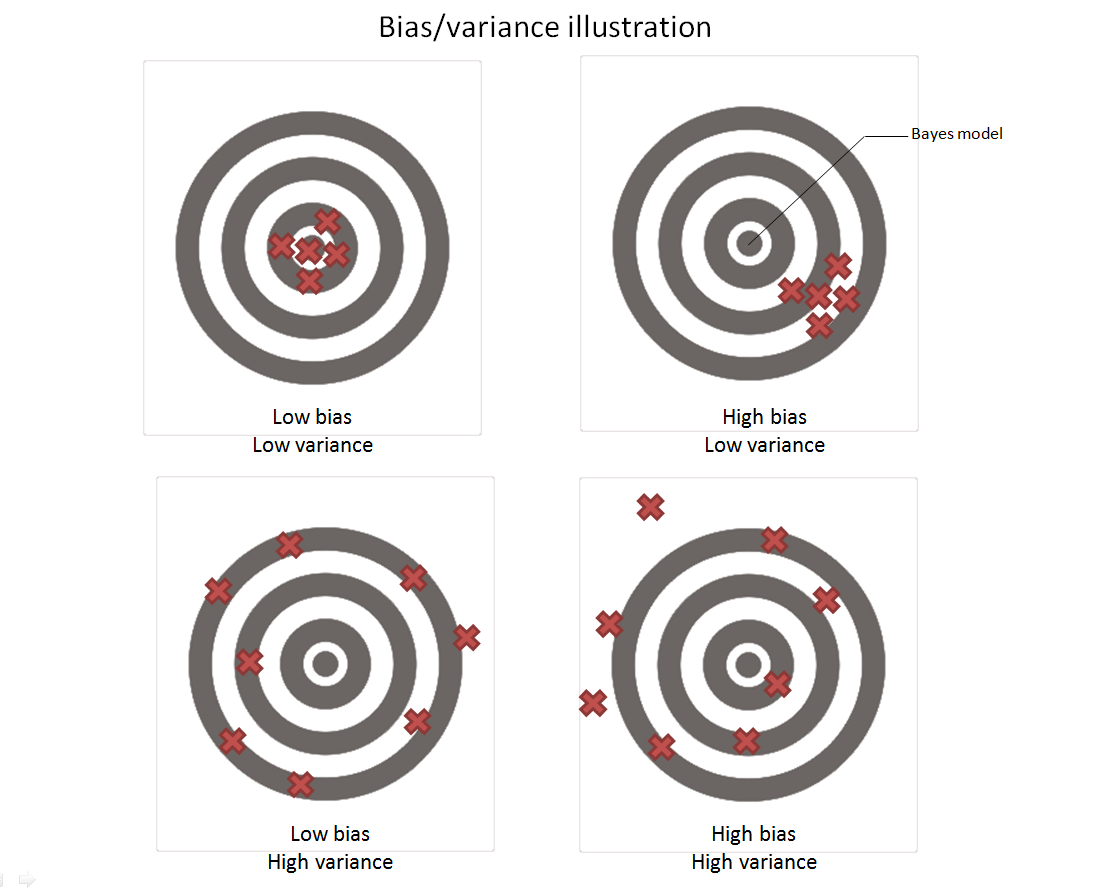
\includegraphics[width=0.7\textwidth]{images/BiasVariance.png}
	\caption{\label{fig:BiasVariance}Bias/variance schematic illustration}
\end{figure}

\paragraph{}
The space of candidate model $\mathcal{H}$ is composed of elements of varying complexity. For instance, a decision tree complexity is assessed by its number of nodes. A more complex model will fit the learning set better, thus reducing the resubstitution error. However, fitting this set too well will cause overfitting : the algorithm incorporate set-specific details. This is reflected by the model variance term of the learning algorithm's error decomposition : slight changes in the learning set will produce very different models. The bias decrease will, at first, overcompensate that increase, yielding a better generalization error. The compensation will work up to the point where the average is of the same order of complexity as the Bayes model. From that point on, the bias decrease will slow down while the model variability continues to increase. Therefore, the generalization error starts to increase as well.
\par
The ability to control the complexity is an important characteristic of a learning algorithm. Another way around this problem is to resort to \textit{ensemble} techniques. Among such are methods which combine several models by averaging their predictions. The models are usually drawn from the same candidate space by either using different learning set or introducing some randomization in the learning algorithm, sometimes both. Ensemble methods rely on the averaging to reduce variability and thus can enjoy more complex models. Ensemble of decision trees form classification forests.
\paragraph{}
A learning algorithm is usually dependent of some parameters, which influence the optimization strategy. They are called hyper-parameters so as not to confuse them with the other parameters on which the optimization is performed.

\section{Image classification}
Traditional learning algorithms are not able to works with ``structured data'' such as texts, images and graphs. Indeed, they expect the individual features to be scalar. Image classification is therefore much more about bridging the two realities than about developing brand new learning algorithm. We will now review the main such techniques.

\paragraph{}
A first way of approaching image classification would be to define descriptors and build a set a rules, in one form or another, so as to discriminate accordingly the images on basis of those descriptors. A first step toward supervised learning is to delegates the construction of the set of rules to a learning algorithm. This had already been successfully attempted back in the 80s (\cite{earlyDecisionTree}, for instance). Since these first incursions of supervised learning in the domain, the interest for them and their achievements have not stopped growing. 
\par
A major concern of the field is dedicated to the image descriptors. Be they structure, spatial, spectral, color or texture descriptors, they actually are the part which bridges the image classification with the supervised learning framework. Moreover, the classification task is only as good as the descriptors allow. The extent to which defining the descriptors must be included in the learning process is still an open debate today. 
\par
On the one hand, learning the descriptors allows for a fully generic approach. In this case, the descriptors and rules are usually learned together by the learning algorithm. This can be done by supplying the image in the coarsest acceptable form to the learning algorithm. This is usually done by vectorizing the image in some fashion, in row prime order for instance, so that feature vectors are composed of the raw pixels. This representation is not lossless, however, as some of the spatial structure is lost in the process. Even resorting to better spatial indexation scheme, such as Hilbert or Peano curves, does not help ; the problem lies in the learning algorithm which have not been designed to incorporate directly spatial relationships. Not all this information is lost, though, but rather presents itself in the form of correlations instead of spatial autocorrelations. Whether or not this can be exploited is algorithm-dependent. From now on, we will designate this approach by ``raw-pixels''.
\par
On the other hand, we find custom descriptors, which are derived from the images. Such descriptors have two advantages compare to the previous ones. Firstly, they are usually less numerous, meaning that the problem is cast to a lesser dimensional space. These are usually easier and more efficiently solved. The second advantage is that they can focus on relevant information regarding the classification task. This last characteristic hides the main drawback of this scheme : information fed to the learning is biased and can miss some important information. So as to limit these side effects and keep some generality, the descriptor can stay at a reasonable level of abstraction. Example of this is using an histogram as descriptor (\cite{histoIntersectSVM}). Concerning the spatial structure, it is \textit{de facto} lost but can be purposefully reintegrated in the form of dedicated descriptors (see for example \cite{geostat}). From now on, we will designate this approach by ``custom descriptors'' or representation learning.

\paragraph{}
In decades of investigation, the scientific community has been prolific on the topic. Therefore, we will focus on several interesting techniques instead of making a detailed tour of the subject.
Three such methods, relating to the present work, will be inspected : Pixit, bag of visual words and convolutional neural network.

\subsection{\label{subsec:Pixit}Pixit}
This raw-pixels classification scheme was introduce in \cite{pixit}. Pixit consists on extracting patches from the original images to build a second database with more objects. The subwindows can either have a predefined, fixed size or can be drawn randomly, possibly within a range of predefined sizes. In the latter case, the patches must be rescaled to a fix size before being described by their raw pixel values so as to form a coherent learning matrix. It is possible to apply other transformation to the subwindows so as to introduce invariances in the learning set, for example towards rotations (\cite{recapPixit}). In case of multicolor images, the method offers to work either in the RGB or HVS color space. 
Once computed, the learning matrix can be fed to any classifier, yielding one class per subwindow. Attributing the final class to the original images is done by voting over their subwindows.
\par
Depending on the patches' size and the number of colors, the feature vectors can be long. Such high dimensionality is not easy to cope with for all the learning algorithm. That is why they envision a tight coupling between the subwindow extraction and a tree-based classifier. On the one hand, enlarging the data in this fashion allows to build more complex models require to cope with the high dimensionality imposed by the raw pixel representation. On the other hand, decision tree and classification forest do not suffer as much from long feature vectors as other might. This is especially true regarding the computational learning cost of their choice of classification forest, namely extremely randomized trees.
\begin{leftbar}
	\paragraph{Ensemble of extremely randomized trees (ExtraTrees)}
	\paragraph{}
	They were introduce in \cite{extratrees} and resemble random forest (\cite{randomforests}). In both kind of forests, only a subset of the features are examined at each node to determine the splitting criterion. This approach is called local random subspace and was introduced in \cite{randomsubspace}. 
	\par
	They differ in the following way : while random forests use bagging as an extra mechanism to introduce randomness, the ExtraTrees determine the splitting thresholds randomly. Bagging, for bootstrap aggregating, is the fact of drawing with replacement several learning samples from the original one (boostrap) and combining their predictions (aggregating). 
	\par
	The advantage of ExtraTrees over random forests is threefold. Firstly, the bagging introduces an effective reduction of the learning size of 36\% for each tree. This is not the case of the ExtraTrees, where all trees can learn from the whole learning sample. Secondly, they are much faster to build since we do not need to pick the optimal splitting thresholds of all the variables examined in a node. Lastly, they tend to perform better than their counterpart (\cite{extratrees}).
\end{leftbar}
The method has been extensively studied in the domain of image classification (\cite{base}). It can go beyond this field, though. In \cite{PixitImgRetrieval}, they venture in the field of image retrieval by developing a similarity measure thanks to both the subwindows and the ExtraTrees. In \cite{PixitLabeling}, they turned to image annotation, \textit{i.e.} pixel-wise labeling. By examining the correctly classified subwindows, it is possible to visualize region of interests and thus get insight about the classification task. In essence, generating many subwindows is akin to producing local descriptors, although it is unlikely that they will all have the same usefulness. This shortcoming can be overcome by supplying control information, so as to automatically discard irrelevant subwindows.



\subsection{\label{subsec:BagOfVisualWord}Bag of visual words}
%Bridge back and forth : ECR and zebra-fish
Bag of words takes its root in text classification. As texts are structured objects, like images, they also need descriptors. A common practice is to represent them by an histogram over the words they contain ; a bag-of-word descriptor. Formally, a bag, or multiset, is a pair $(S, n)$, where $S$ is a set and $n : S \rightarrow \mathbb{N}_+$ is a numbering function. Representing several texts is done by establishing a reference dictionary $S$, specifying an ordering of the words and counting how many times each appears in a given text. Common words are usually discarded so as to focus on specific vocabulary. As we can see, no spatial information is kept.
\paragraph{}
The same principle can be applied in image classification, leading to custom descriptors. The main difficulty lies in the fact that the set of so-called ``visual words'', \textit{i.e.} the dictionary, is not known in advance, or well defined, for that matter. Consequently some preprocessing is require to come up with the dictionary. The most popular solution relies on interest point detection followed by vector quantization (\cite{BagOfWords}). 
\par
Interest point detection is usually carried out by the Scale Invariant Feature Transform (SIFT) method (\cite{SIFT}, \cite{SIFTExplained}) or its PCA variant : PCA-SIFT (\cite{PCASIFT}). They work by locating ``keypoints'' : points of interest stable with respect to scale and orientation shifts. The keypoints are then described by a normalized histogram of orientation gradient in the form of a 128 element feature vectors, for the traditional SIFT and in a more compact variant for the PCA-SIFT.
\par
Processing the images will lead to a set of different keypoints and cardinality, just as texts were composed of different words and of varying length. We thus have to fix a dictionary, and by extension an ordering of the words. The situation is slightly different than in the text situation because minor variation of a given keypoint descriptors are possible, whereas, spelling mistakes aside, this is not the case with texts. This is where vector quantization comes into play. During the learning phase, a given number of prototypes are constructed by way of the K-means clustering algorithm. The prototypes are the visual words and form the dictionary. The ordering is arbitrary but must be fix once and for all by assigning an index number, or position, to each prototype. Once this dictionary has been built, each learning keypoint is associated to the closest visual word. Then an histogram is built for each image by counting all its visual words. These histograms constitute the learning matrix, which can be fed to any learning algorithm. Classifying a new image is done symmetrically : the keypoints are detected, they are assigned to a visual word and the histogram word is computed to form the feature vector, which can then be fed to the classifier.
\paragraph{}
An important bridge between this and the Pixit method was raised by \cite{ETFL}, in the form of extremely randomized clustering forests (ERC-forests). Although anchored in the bag of visual words framework, they switch the SIFT keypoints detection for an iterative mechanism involving random subwindows. As for the dictionary construction, it does not rely on K-means any longer but rather on extremely randomized trees. The dictionary words are composed of $T$ parts of different sizes, where $T$  is the number of trees.
Each part encodes the index of the leaves where a given object ends up in a one-hot fashion. Thus, the part corresponding to a tree with $L$ leaves will be a binary word with $L-1$ zeros and $1$ one. Once again, the final features vector of a given images is the histogram computed over all the subwindows belonging to that image.
It was later incorporated in the Pixit framework, although without the iterative loop regarding the extraction of patches in order to fit better in the framework. This mechanism is sketched at figure \ref{fig:ETFLHisto}. 
\par
In this context, it is known as ET-FL (ExtraTrees for feature learning) by opposition to ET-DIC (ExtraTrees for direct image classification). This variant was thoroughly studied in \cite{base}. They show that, in most cases, the ET-FL approach performs slightly better (3-4\% in average). Nevertheless, ET-FL is more difficult to tune.


		\begin{figure}
			\begin{subfigure}{.5\textwidth}
				\centering
				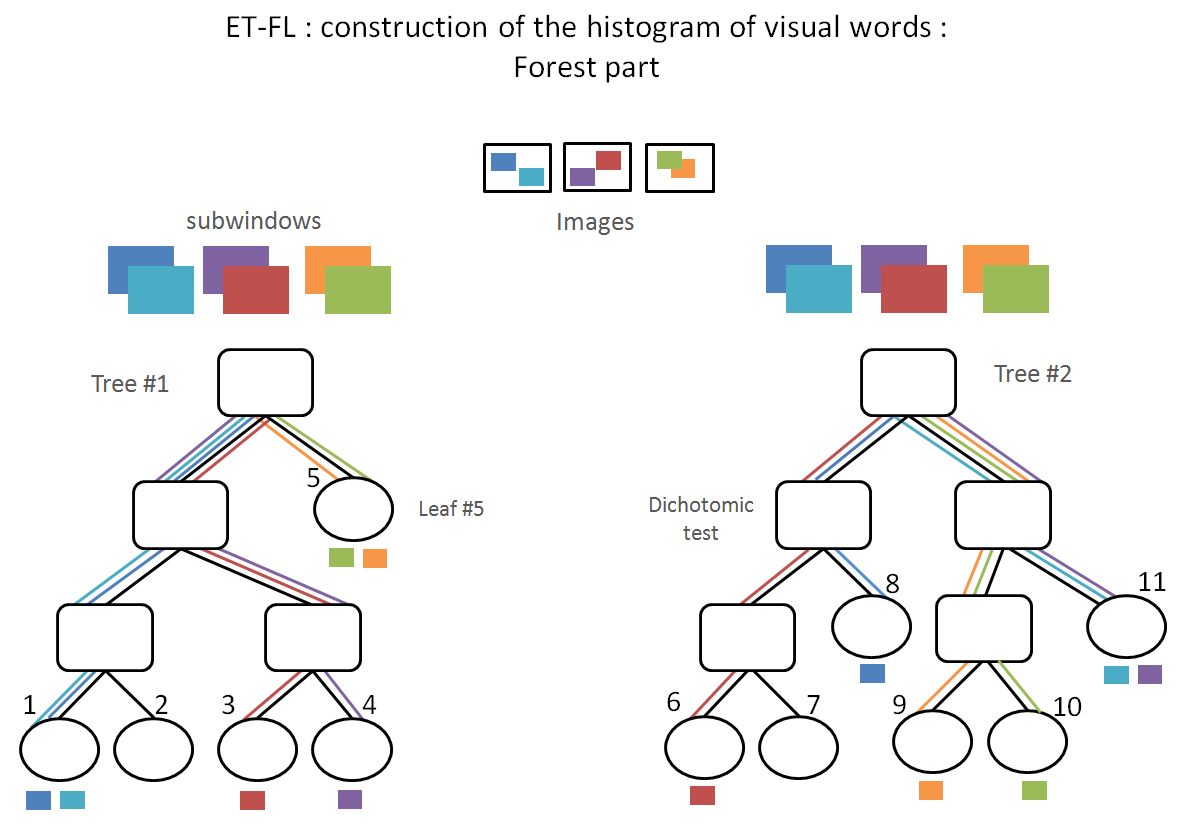
\includegraphics[width=1.\linewidth]{images/ETFLHisto1.png}
				\caption{\label{fig:ETFLHisto1}}
			\end{subfigure}%
			\begin{subfigure}{.5\textwidth}
				\centering
				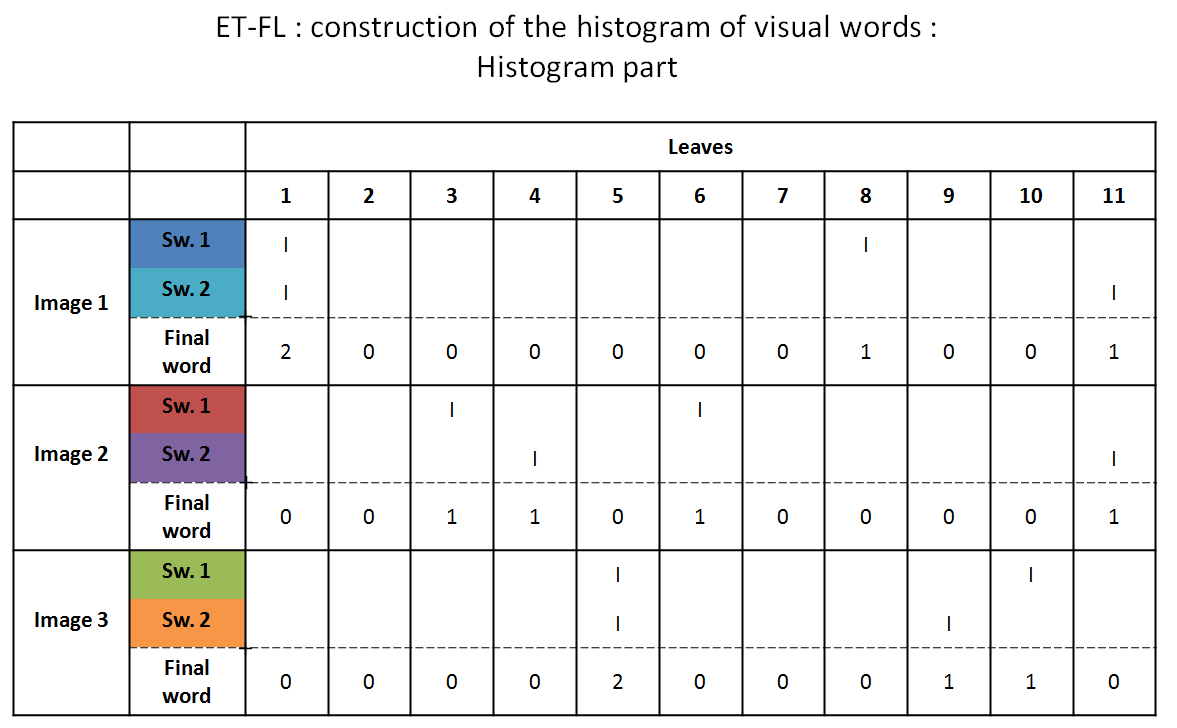
\includegraphics[width=1.\linewidth]{images/ETFLHisto2.png}
				\caption{\label{fig:ETFLHisto2}}
			\end{subfigure}
			\caption{\label{fig:ETFLHisto}Creation of the histogram words}			
	\end{figure}
	
		In both ET-FL and ERC-forests cases, the actual classifier is a support vector machine (SVM).
		\begin{leftbar}
			\paragraph{Support Machine Vector (SVM)}
			\paragraph{}
			Support machine vector take their roots in the work of \cite{svm} and were originally designed as linear classifier for linearly separable tasks. A dataset with binary classes is said to be linearly separable if it is possible to draw an hyperplane in the space of regular features which ``separates'' the two subsets of data.
			More formally, the hyperplane $H_{w,b} = \{x \in \mathbb{R}^n | w^T x = b\}$ with $w \in \mathbb{R}^n$ and $b \in \mathbb{R}$ separates two points $x_1$, $x_2 \in \mathbb{R}^n$ if and only if 
			\[
				(w^T x_1 - b)(w^T x_2 - b) < 0
			\] 
			Let us note that, with this definition, if two sets are separable, there is an infinity of separation hyperplanes. The goal of the SVM is to choose the one which produces the biggest margin : to maximize the minimum distance from any point of the dataset to the hyperplane.
			\par
			So far, the SVM suffers from three limitations. Firstly, it can only tackle linear problems. Secondly, it is restricted to the class of separable problems. Lastly, it is further confined to binary classifications. 
			\par
			The first problem can be overcome either by deriving new features through functions of the original ones or via what is known as the ``kernel trick''. All the computations involving the data are actually inner products. Therefore, one can use any such product instead of the standard scalar one. 
			\par
			Overcoming the linear separability is done by introducing slack variables that allows for points to be inside or even cross the margin, behavior which is penalized in the objective function. This soft margin formulation was proposed by \cite{svmsoft}.
			\par
			As for the last limitation, several ways around have been proposed and discussed in the literature (see \cite{svmmulticlass}, for example). A common scheme is the one-versus-all. 
		\end{leftbar}



\subsection{Convolutional neural network}
%Box neural network \cite{ConvNet} <-- zip code
Convolutional neural networks (convnets or CNNs) were first introduced in the context of zip code recognition \cite{ConvNet}. This raw-pixels technique is a special case of neural network.
\begin{leftbar}
	\paragraph{Neural network}
	\paragraph{}
	The perceptron model was introduced by \cite{perceptron}. It is based on a two layer network of ``neurons''. A neuron's goal is to come up with a separating hyperplane. Unlike SVM, the hyperplane might not maximize the margin. Indeed, the hyperplane optimization is carried by (stochastic) gradient descent, implying that the learning can be done online. Online learning, by opposition to batch learning, do not require to have the whole dataset in memory. A sigmoid-like function usually encapsulate the hyperplane so as to introduce non-linearities in the model.
	\par
	The creation of the backpropagation algorithm (\cite{backpropagation}) allowed for the creation of more complex networks called multi-layer perceptron (MLP). The backpropagation allows for each neuron to learn its local model with the only need of neighbors' information. It is a two-phase algorithm. During the forward pass, the hyperplane coefficients are known and a global output can be computed by propagating the input through the network. The error can then be computed and a correction is applied to the last layer. Then a compensation can be applied to the previous layer and so on up till the first layer. 
\end{leftbar}	
Convnets hold the accuracy records on a variety of image classification benchmarks and contests (\cite{ImagenetRecord}, \cite{convnetRecord} and \cite{bestcifar}, for instance). They differ from regular neural networks in the two ways.
\par
Firstly, their numerous layers are partitioned into two categories. The lower layers are not fully connected while the uppers, if any, are. The partial connectivity is not made at random but rather enforces that the neurons work on spatially local information. The neurons of a given low layer are partitioned into subsets, also called feature maps. Each element of a subset shares the same spatial weights and together cover the whole input image with a great amount of overlapping, hence their name. So far, the input of layer $k$ is the output of layer$k-1$ ; several images (one per feature map) ultimately derived from the original image. Since the different layers are designed to work at different spatial scales, the level of detail of the previous layer is usually not required. Therefore, the image is usually undersampled rather than working with bigger feature maps.
\par
Secondly, a a function of spatial pooling is introduced between the layers. It consists on aggregating the results spatially close feature maps. It serves two purposes. The first one is to introduce translation invariance and other spatial robustnesses in the model. Indeed, the exact position of a given characteristics is usually much less important than knowing whether or not it appears. The second goal of the spatial pooling is linked to the undersampling between layer : it prevents that mechanism to miss an important characteristic by a poor choice of pixels. Usual spatial pooling functions are the average and maximum. The latter usually serves as presence/absence detector and introduces more non-linearity in the model. In any case, the undersampling and the spatial pooling can be conducted at the same time by defining a neighborhood window : neurons of the same feature maps which fall into the neighborhood window aggregate their results together an produce a common output. Depending on how the neighborhood windows overlap, the change in resolution might be important or not.


\paragraph{}
As we can see, the network complexity is substantial. For example, in the case of the zip code problem (\cite{ConvNet}), there are already 2592 parameters to optimize even though there is only 12 feature maps and three layers. Nowadays problems account for much greater complexity. Consequently, running time of convnets are usually important. Fast and efficient GPU implementation are now available (\cite{GPUConvnet}) but one has also to take into account the time necessary to optimize the network structure and other hyper-parameters, a much more complex task. As far as accuracy is concerned, convenets is the best. However, they are not really practical solutions, as yet. Numerous work in the field of optimization are currently helping with these issues, with remarkable success. Nevertheless, we are not yet in a situation where convnets are turnkey solutions, situation which may well never happen. 
\par
In the meantime, at the least, it would be nice to dispose of a solution which combine convnets accuracy with ease-of-use of, say, the Pixit method. Such a method would also allows to bridge to the bag of visual words framework through the ET-FL mode of the Pixit. Producing this missing link is the central objective of the present work. How we propose to proceed will be made clearer in the next chapter.
%Missing link
%Cite other stuff


%==========================================================================================================================================
\chapter{Objectives and methodology}
In this brief chapter, we lay down our objectives, methodology and contributions.

\section{Objectives}
The hypothesis at the core of the present master thesis can be stated as follows : 
\begin{quote}
It is possible to combine the advantages of the classification forests, namely computational cost, feature importance evaluation and ease of use, with those of convolutional networks, primarily the accuracy.
\end{quote}
\paragraph{}
%TODO : Come back to the computational cost and see how long it takes for the winners
The feature importance evaluation capability is one of the nicest features of the classification forests. The importance of a given feature is computed as the total reduction of impurity brought by that feature, normalize so that the feature importances sum to one. The most notable use of this measure is for feature selection. Focusing on a smaller set of features is computationally more tractable, can provide better accuracy when the other features are irrelevant and can bring more insight to the classification problem.
\par
The ease of use of the forests is particularly obvious in comparison with the neural networks, for instance. With the former, the number of hyper-parameters is quite small and well understood. Therefore, tuning the method is easy and can, usually, be undertaken manually with good results. Besides, the default parameters usually performs well enough. On the other hand, neural networks tuning is much more complex, as even the structure has to be adapted for each problem. Evidence of this complexity is the amount of work dedicated to this subject in the literature. %Ref Geurts et opti
\par
%Convolutional network accuracy is state of the art, blabla \par
Lastly, let us mention an interesting characteristic of convolutional networks we did not pursue but which has an important impact on scalability : online learning. Indeed, classification forests require to have the total amount of data right away which may be a limitation of our method.


\section{Methodology}
\subsection{The RandConv algorithm}
Validating the hypothesis constitutes our main objective. To achieve this, we developed a method named RandConv based on classification forests which incorporates some convolutional networks mechanics. More specifically, random linear filters are applied to the image database, followed by one or several spatial pooling(s). Then, several random subwindows are extracted from each processed image. Each subwindow is described by the raw pixel values. The method is thus divided into the following parts :
	
	\begin{enumerate}
		\item Generating the $N$ linear filters
		\item Applying the $N$ filters to the $M$ images of the databases
		\item Applying the $P$ spatial poolings to the $N \times M$ filtered images
		\item Extracting $S$ subwindows from each of the $N \times M \times P$ pooled and filtered images and resizing them
		\item Describing each of the $N \times M \times P \times S$ pieces by a set of $F$ learning features each
		\item Reorganizing the data to create a $(M \times S) \times (F \times (N \times P))$ learning matrix
	\end{enumerate}
	
	
	The pseudo code is presented by algorithm \ref{algo:RandConv}. The algorithm can be parallelized easily by subdividing the image dataset in several pieces and reassembling the learning submatrices accordingly. It is also intended to be able to use the original image as if the first filter was the identity filter. The poolings, however, are still applied to it.
	
	
	\begin{algorithm}
		\caption{\label{algo:RandConv}RandConv extraction algorithm}
		\begin{algorithmic}[1]
			\Procedure{process}{$RandConvInstance$, $images$}
				\State $rci \gets RandConvInstance$
				\State $N \gets rci.nbFilters$
				\State $P \gets rci.nbPoolings$
				\State $S \gets rci.nbSubwindows$
				\State $F \gets rci.nbFeaturesPerSubwindows$
				\State $M \gets images.length$
				\State $\textit{learningMatrix}[M \times S][F \times (N \times P)]$
				\State $row \gets 0$
				\State $colMin:colMax \gets 0:F$
				\For{$image \in images}$
					\State $cropboxes \gets rci.generateSubwindowLocations()$
					\For{$filter \in rci.filters$}
						\For{$pooling \in rci.poolings$}
							\State $filtered \gets rci.applyFilter(filter, image)$
							\State $pooled \gets rci.applyPooling(pooling, filtered)$
							\For{$cropbox \in cropboxes$}
								\State $subwindow \gets rci.extractSubwindow(cropbox, pooled)$
								\State $learningMatrix[row][colMin:colMax] = rci.describe(subwindow)$
								\State $colMin:colMax \gets colMax:colMax+F$
							\EndFor
						\EndFor
					\EndFor
				\EndFor
				\Return $learningMatrix$
			\EndProcedure
		\end{algorithmic}
	\end{algorithm}
	
	
The in-depth description of this RandConv method is the main subject of chapter \ref{chap:RandConv}.
	This method builds on previous works. The idea of applying predefined convolutional filters followed by several spatial poolings before extracting subwindows has already been done in \cite{base}. It constituted a generalization of their generic image classification scheme (\cite{pixit}), called Pixit. 
	
	
	\subsection{Dataset and environment} %TODO : cite GIGA computer
	%CIFAR-10 : Several important results. 288 Go de ram dont 145 en shm. 30 core. frequency ?
	We will be working with the CIFAR-10 database (\cite{cifar}). This dataset is composed of a learning set of 50,000 images and a testing set of 10,000 images. They are grouped into 10 mutually exclusive classes : airplane, automobile, bird, cat, deer, dog, frog, horse, ship and truck. Both subsets contain an equal number of images from each class. The images are of size 32x32 and are RGB.
	\par
	This database has been chosen because it was the same one on which the precursory method from \cite{base} was tested. In turn, they chose this dataset because their traditional solution had difficulties with it. 
	\par
	The best result on this database is an accuracy of 91.2\% and is hold by a convolutional network (\cite{bestcifar}). The top ten best results are above 80\%. Most are neural network solutions and none are based on classification forests.
	\paragraph{}
	The learning and testing will be carried out on a 64-bits 30-core 2.1 GHz computer with 288 GB of RAM from the Cytomine project (\cite{cytomine}) and GIGA bioinformatic platform.
	
	
	\section{Contribution}
	The contribution of the current paper is twofold.
	\par
	Firstly, the RandConv framework proposes several extensions of the precursory method, the most noticeable of which being the ability to generate the filters randomly. This approach resembles more the convolution networks, where the filters are actually learned.
	\par
	Secondly, whereas the aforementioned work was a proof of concept, the present study aims at analyzing more deeply this method. Indeed, proving the hypothesis is not our only goal. We also want to study closely the behavior of our classification method so as to understand its strength and limitations. This is the focus of chapter \ref{chap:results}.
	\par
	The present works differs from \cite{NearlySame} in three ways. Firstly, the randomly generated filters are not used in the same fashion. Whereas they use them as a randomization mechanism to introduce variability in the trees, we incorporate them all for each trees of the forest so that the individual trees will \textit{choose} which filter to emphasis. Secondly, we are using a layer of spatial pooling missing in the aforementioned paper and extracts several subwindows instead of working with the whole image directly. Finally, we work at a much bigger scale, providing at least several tens of filters to the forest. 

%==========================================================================================================================================
\chapter{\label{chap:RandConv}The RandConv framework}
This chapter is divided into three sections. The first one aims at fully describing our classification method. The second section highlights implementation details and technical issues. The last one summarizes the hyper-parameters and fixes their default values.

	\section{RandConv components}
	This section is dedicated to an in-depth description of our classification method : RandConv. It stands for ``Random and 	convolutional''. The ``random'' part refer to both the filter generation and subwindow extraction. While the ``convolutional'' adjective refers to the application of the linear filters. 
	\paragraph{}
	So as to bridge between classification forests and convolutional networks, we started from the former and added characteristics of the latter. Those characteristics are the convolutional filtering followed by spatial pooling.
	Although, the method has been designed with the use of classification forest in mind, the RandConv method, \textit{per se}, is actually a feature extraction method. Its goal is to transform a set of images into a set of corresponding feature vectors. The actual classification could be carried out by any traditional learning algorithm. Nevertheless, regarding our primary objective and some other attractive properties of the trees, which will be developed shortly, we will stick with classification forests in one way or another.

	
		\subsection{Filter Generation and application}\label{subsec:methodo-filtergen}
		%dimension, square size, odd natural, uniform at first
		%coefficients
		Mimicking the convolutional filtering is carried out by generating random linear, spatially invariant filters. More precisely, we generate the 2D finite impulse response matrices. First, the filter dimensions and then the filter coefficients are randomly drawn. This means that, contrary to the ConvNet, the coefficients are not directly learned. The coefficient learning is simulated by generating a vast number of filters and letting the learning algorithm choose the ones to emphasis. 
		\par
		This calls for an important remark : decision-tree-based solutions are ideal classifier candidates. Firstly, their construction technique allow them to emphasis easily the interesting filters. Secondly, they deal well enough with numerous, possibly irrelevant, features. Indeed, the major impact is a reduction of the model effective complexity. The resulting accuracy drop is much less tremendous than with some other classifiers. Besides, this reduction of complexity can be balanced by the number of subwindows extracted from each image. Augmenting the dataset produces deeper trees ; more complex model. Lastly, they scale well enough due to their relatively low computational cost, especially the extremely randomized tree variant.
		
			
			
			\subsubsection{Drawing mechanism}
			How to draw the filters is one of the RandConv framework cornerstone. The drawing mechanism should meet two requirements. Firstly, it should be able to produce unlimited, or at the least, a great number of different filters. Secondly, the filters should be of some value by themselves but also together. Intuitively, a valuable filter should highlight ``information'' not directly accessible from the original image by the learning algorithm. We will call this characteristic the individual usefulness or simply usefulness. As for having value together, two different filters should not uncover the exact same ``information''. For instance, producing twice the same filter is useless. We will call this the group usefulness or co-usefulness.
			
			\paragraph{}
			Several drawing mechanisms have been developed with different motivation in mind :
			
			\begin{itemize}
				\item Custom filters
				\item Discrete law generator
				\item Zero-perturbation generator
				\item Identity-perturbation generator
				\item Maximum-distance-from-identity generator
				\item Stratified perturbed generator
			\end{itemize}
			
			The first one is a special case. It consists of a set of 38 well known filters, among which the Sobel and Prewitt filters, several Laplacian filters of different sizes, the compass gradient filters, some low and high pass filters and other line detection filters.
			%\begin{multicols}{3}
			%\end{multicols}
			Being a small set, it violates the first prerequisite. However, this pseudo filter generator will be useful as a comparison basis : the filter are the same ones as in \cite{base}. Besides, these filters have practical application cases which random filters might not share. It is thus a reference point to see whether the generated filters highlight interesting ``information''.
			\paragraph{}
			The other mechanism draw the filters randomly. Before generating the coefficients of a filter, its dimensions must first be determined. The widths and heights of the impulse response matrices are drawn from an bounded set of odd, positive integers. Although we limited our tests to square matrices, this is not a strict requirement.
			\par
			We mainly worked with a uniform distribution of sizes, playing somewhat with the set bounds. Once again, this is not a limitation as other distribution can easily be used. For example, it is possible to create a distribution biasing towards small sizes. 
			\par
			As for the bounds, the minimum was fixed to 3. The maximum size needs probably not be greater than half the image size. Indeed, greater filters might incorporate mostly global information and provides too much redundancy.
			\par
			Conceptually, for a given maximum size, say $n = h \times w$, it is easy to build a bijection between the filter matrices space and $\mathbb{R}^n$. This representation will help us visualize the drawing mechanisms.
			\paragraph{Discrete law generator.}
			Once the size is fixed, every coefficient is drawn for a predefined discrete law. Even though the number of such filters is bounded for a given maximum size, this filter space is still vast enough so as to meet the first generator prerequisite. We tested the following law : -1 with a probability of .3, 0 with a probability of .4 and 1 with a probability of .3.
			This generator was motivated by the spatial interpretation of the convolution. It accounts to summing and subtracting neighboring pixel together.
			\paragraph{Zero-perturbation generator.}
			Once the size is fixed, every coefficients are drawn from the same continuous probability law. Although there is no restriction on the probability law, we expect it to be symmetrical and zero-centered, hence the generator name. We used two such laws. The first one is the uniform law over reals bounded with -1 and 1. In this respect, the generator space is mappable to an hypercube centered on the origin. The second law was a Gaussian so that the probability of being outside the range [-1, 1] is equal to a given threshold. The isoprobabilities thus form hyperspheres. The points lying outside of the range can be forced to the boundary so that the generator space becomes the same hypercube as with the uniform law. 
			Zero-centered generator were motivated by the examination of common filters which portray the same characteristic.
			\paragraph{Identity-perturbation generator.}
			Identity-perturbation generator work in the same fashion as its zero-perturbation counterpart. The only difference is that the hyper-structures are centered around the identity filter instead of the origin. 
			The motivation behind this generator was to produce filtered images resembling the original while being different enough so as to be of value.
			\paragraph{Maximum-distance-from-identity generator.} 
			This kind of generators fulfills the same purpose as the previous one. The generator space is also centered on the identity filter but its shape is different. We decided to work with the Manhattan distance. Concretely, the generator is parametrized by a maximum distance, independent of the filter sizes. The coefficients are processed in a random order. A random perturbation from the range $[-maxDist, maxDist]$ is applied to the first coefficient. Before processing the next coefficient, the maximum distance is updated by subtracting the absolute value of the perturbation.
			\paragraph{Stratified perturbed generator}
			This last class of generators are parametrized by a minimum value $m$, a maximum value $M$ and a subdivision number $n$. For each coefficient, a value $v$ from the set $\{m + \frac{k+1}{2} \times \frac{(M-m)}{n} | k \in \mathbb{Z}, k < n\}$ is chosen randomly.  This value is then randomly perturbed before being assigned to the coefficient. The perturbation is not mandatory and should stay in the range [$-\frac{(M-m)}{2n}, \frac{(M-m)}{2n}$]. Expected perturbation law are Gaussian and uniform. This is illustrated by figure \ref{fig:stratgen}
			\begin{figure}
				\centering
					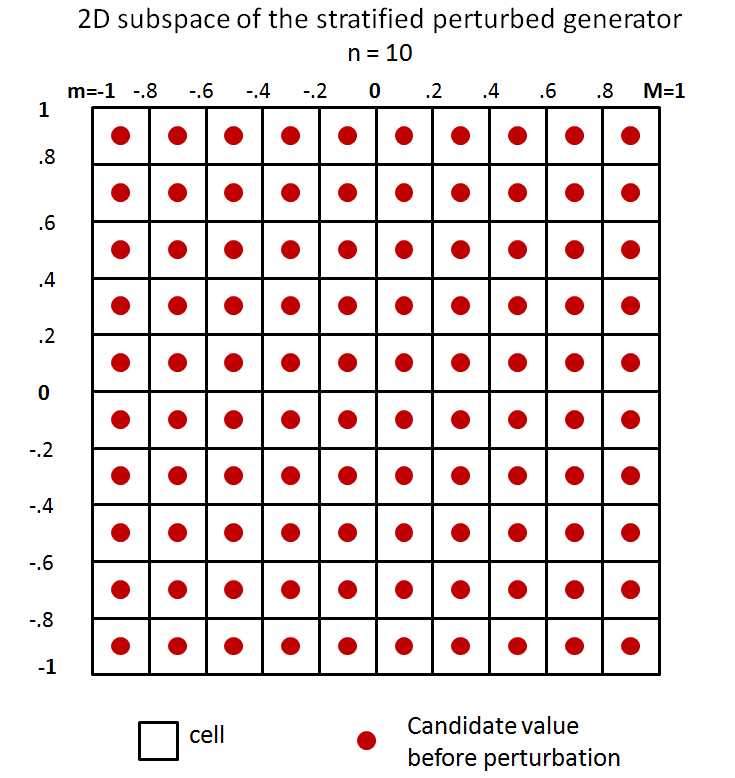
\includegraphics[width=0.5\textwidth]{images/stratgen.png}
				\caption{\label{fig:stratgen}2D cut in the stratified generator space (10 subdivision between -1 and 1, no perturbation)}
			\end{figure}
			
			\par
			This generator class was motivated by the idea to produce as dissimilar filters as possible so as to meet our second requirement about co-usefulness. Disregarding the perturbation, the filter space is finite but still huge. For instance, the space for a subdivision number of 10 with only the smallest filters (3x3) would still mean $10^9$ filters.  Whereas $2^9$ filters, \textit{i.e.} a subdivision number of 2, is manageable, the other generators are able to produce filters as dissimilar. Furthermore, the following non-monotonicity property suggests that a dissimilar approach in the filter space might not be the best way to produce sets of co-useful filters. Indeed, one way of assessing co-usefulness is to use a distance measure : if two filtered images are close, they probably highlight the same ``information''.
			
			\paragraph{Non-monotonicity property.}
			We will show that closeness in the filter space does not necessarily imply closeness of the filtering results. Closeness is to be understood as distance from a reference.
			Let $I$ be an image and $F$, $F_1$, $F_2$ be three linear, spatially invariant filters of possibly different sizes. Let also
			\begin{align*}
				J &= I * F \\
				J_1 &= I * F_1 \\
				J_2 &= I * F_2 \\
			\end{align*}
			We will show by counterexample that $\parallel F - F_1 \parallel \geq \parallel F - F_2 \parallel \centernot\implies \parallel J - J_1 \parallel \geq \parallel J - J_2 \parallel$.
			First let us name $e_1 = F - F_1$ and $e_2 = F - F_2$. By linearity of the convolution, we have :
			\[
				J_1 = I * F_1 =  I * (F - e_1) = (I * F) - (I * e_1) = J - (I * e_1)
				\iff
				J - J_1 = I * e_1
			\]
			In these terms, we have to show that $\parallel e_1 \parallel \geq \parallel e_2 \parallel \centernot\implies \parallel I * e_1 \parallel \geq \parallel I * e_2 \parallel$. 
			Let us take $e_1$ such that the coefficients sum up to zero but with a great dispersion (a Sobel filter, for example) and $e_2$ such that the sum of the coefficients is strictly greater than zero but with a smaller dispersion than $e_1$ (the 3x3 average filter, for instance). Thus, we have  $\parallel e_1 \parallel \geq \parallel e_2 \parallel$. Moreover, let us consider the case of a image $I$ with constant value $c > 0$. In this setting, $\parallel I * e_1 \parallel = 0$ while $\parallel I * e_2 \parallel = c \times k > \parallel I * e_1 \parallel$.
			\par
			Therefore, playing with closeness or dissimilarities in the filter space yield no warranty about the same metrics with the filtered images. However, using the distance as measure of co-usefulness is arguably a poor choice, since close filtered imagess might still highlight different aspects of the original image. Considering this remark, the main shortcoming of the stratified generator is probably that, with respect to the number of generated filters we will use, it  does not produce any significant advantage over other generators.
			
			

			
			\subsubsection{Normalization}
			%Justification, impact on the filter space, spatial interpretation & impact, spectral interpretation & impact
			All the generators we discussed in the previous section are able to perform a post-processing normalization of the filter. There are four normalizations :
			
			\begin{itemize}
				\item No normalization : the post-processing normalization is skipped.
				\item Zero mean : the coefficient values are normalized so that their mean value is null.
				\item Unit variance : the coefficient values are normalized so as to have a unit variance.
				\item Zero mean and unit variance : both the previous. First the zero mean then the unit variance.
				\item Unit sum : the coefficients are normalized to sum to one.
			\end{itemize}
			
			The introduction of the zero mean and unit variance normalizations was primarily motivated by supplying support for learning algorithms other than classification forests. Indeed, their effect is to impose a common dynamics to all the filters. While trees can cope easily with variables of different dynamics, some classification schemes are not applicable is that setting or suffer greatly from it.
			\par
			As for the unit sum normalization, applied in conjunction with a generator producing positive coefficients, it produces ``convex combination filters'' in the following sense : for each step of the convolution, the output pixel value is bounded by the minimum and maximum of the neighboring original pixels (where the neighborhood is defined by the filter size).
			\par
			We will now look at the implication of the normalizations on the generator space. We will reuse the filter representation in $\mathbb{R}^n$ and will denote by $\textbf{1}$ the vector whose coefficients are all $1$.
			
			\paragraph{Zero mean normalization.}
			In $\mathbb{R}^n$, the zero mean filters form the hyperplane $\{x \in \mathbb{R}^n | \textbf{1}^{T}x = 0\}$. The normalization is a projection onto that hyperplane. The resulting filter $y$ is computed as $y = x - \frac{1}{n}\textbf{1}^{T}x\textbf{1}$. This operation can produce a filter which is outside of the original filter space.
			Since this operation is linear, the impact of the filtering are straightforwardly identifiable. Denoting $I$ a given image, $x_f$ a given filter, whose mean $m$ form the constant filter $m_f$, $y_f$ the normalization $ y_f = x_f - m_f$ and $\textbf{1}_f$ the constant filter with only ones as coefficients, we have : 
			\[
				I * y_f = (I * x_f) - (I * m_f) = (I * x_f) - m \times (I * \textbf{1}_f)
			\]
			The $(I * \textbf{1}_f)$ correction part is independent of the filter and proportional to the mean coefficient value. The practical impact is clearer in the frequency space. Let us denote by $\rightleftharpoons_\mathcal{F}$ the Fourier transform : 
			\begin{align*}
				I &\rightleftharpoons_\mathcal{F} U \\
				x_f &\rightleftharpoons_\mathcal{F} H_x \\
				m_f &\rightleftharpoons_\mathcal{F} H_m \\
				y_f &\rightleftharpoons_\mathcal{F} H_y = H_x - H_m
			\end{align*}
			\[
				I * y_f \rightleftharpoons W = U \times H_y = U \times (H_x - H_m) = (U \times H_x) - (U \times H_m) = Y - (U \times H_m)
			\]
			Since $m_f$ is a constant signal, the transfer function $H_m$ is null everywhere except at the origin. Thus, the overall frequency response is only marginally modified and both filter achieve the same results.
			Therefore, the normalization does not restrict the class of filters.
			
			\paragraph{Unit variance normalization.}
			In $\mathbb{R}^n$, the unit variance filters form the hypersphere $\{x \in \mathbb{R}^n | x^{T}x = 1\}$. However, in practice, the normalization works with the current filter size and not the maximum filter size. Thus, there are several hyperspheres to consider, one per possible sizes. 
			In the filter space, the normalization equals to scaling the filter so as to meet the appropriate hypersphere. The impact on filtering is immediate :
			\[
				I * y_f = I * (\frac{1}{\sigma_x} x_f) = \frac{1}{\sigma_x} (I * x_f)
			\]
			The whole result is scaled by the same factor. Therefor, the normalization does not restrict the class of filters.
			
			\paragraph{Unit sum normalization}
			The reasoning is identical to the zero mean normalization except for the hyperplane : $\{x \in \mathbb{R}^n | \textbf{1}^{T}x = 1\}$. This normalization does not restrict the class of filters either. 
			
			
			\subsubsection{Filter application}%Border policy for filtering, working with colors
			In this subsection, we cover two topics about the filter application. The first one concerns working with colors. The second one is about how the filter are actually applied. 
			\paragraph{}
			Handling colors can be done in three ways. 
			The first one, is to realize a 3D convolution. This results in a single output value per original pixel. However, there are two drawbacks to this approach. Firstly, in the spatial space, it means combining values of different colors together. This would work but lacks of physical interpretation. Indeed, the RGB space is only a convention. The second drawbacks has to do with the frequency space. It feels awkward to put on a same level spatial frequencies and color frequency, whatever it might mean.
			\par
			The second method to handle colors is to use separate 2D filters on each channel. This produces three values per original pixels. The main drawback of this scheme is that post interpretation of the filters will be difficult.
			\par
			As for the last and simplest method, is to use the same 2D filters on each color. This also produces three values per original pixels.
			Because the last approach seems more natural than the first one and is simpler to interpret than the second, it is the one we adopted.
			\paragraph{}
			Now that we know how to handle colors, let us investigate the filter application.
			The convolution is carried out in the frequency space by multiplying the Fourier transform of the original image by the transfer function of the filter. The output is of the same size as the original image. The borders are handled by padding the original image with zeros.
			
		\subsection{Pooling strategies}
		Now that we have fully covered the filter generation and application mechanisms, we can move on to the next part concerning the spatial pooling strategies. In both cases, we need two elements : a window/neighborhood size and the function to apply on those windows.
			\paragraph{Moving windows.}
			In the case of spatial pooling by moving windows, they are supposed to have odd width and height. The center of the window moves to match every pixel of image. The pooling function is computed on the overlapping part of the window and the image. The resulting image as the same size as the original image. This is illustrated by figure \ref{fig:PoolMW}. 
	\begin{figure}
		\centering
			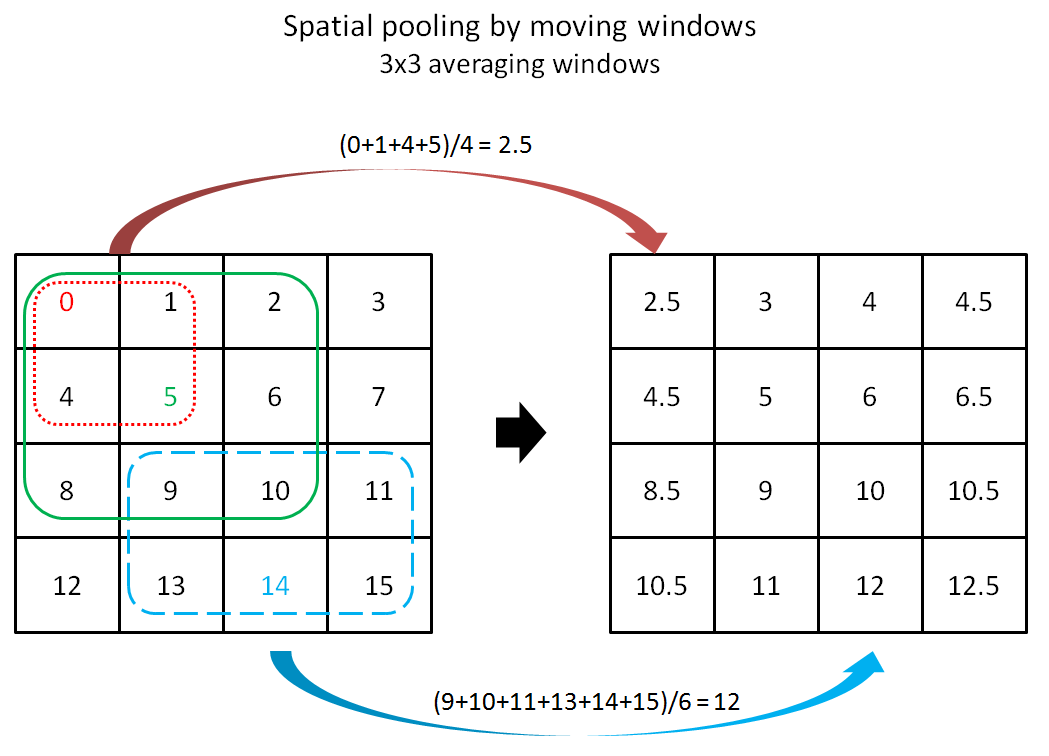
\includegraphics[width=0.7\textwidth]{images/PoolMW.png}
		\caption{\label{fig:PoolMW}Spatial pooling by moving windows}
	\end{figure}
			
			\paragraph{Aggregations.}
			In the case of spatial pooling by aggregation, the neighborhood windows do not overlap. The image is divided into several non overlapping neighborhood such that each neighborhood has the appropriate size. The pooling function is then applied on each cell of this neighborhood grid. Thus, contrary to moving windows, the resulting image is smaller and correspond to the neighborhood grid layout. This is illustrated by figure \ref{fig:PoolAgg}.
	\begin{figure}
		\centering
			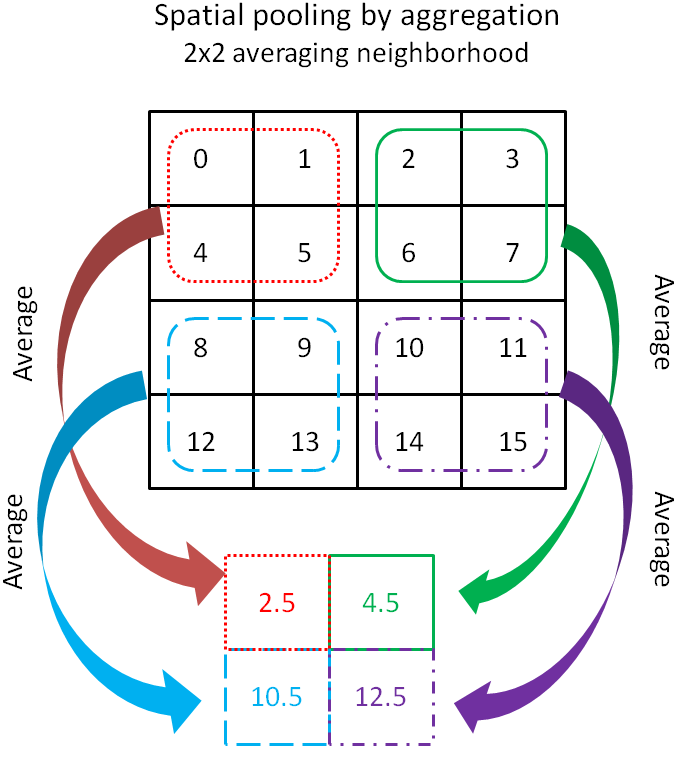
\includegraphics[width=0.5\textwidth]{images/PoolAgg.png}
		\caption{\label{fig:PoolAgg}Spatial pooling by aggregation}
	\end{figure}
	
			\paragraph{Pooling functions.}
			The pooling function box is comprise of the minimum, maximum and average functions. In the case of the average function with moving window, we are close to defining a composition of two linear filters. The difference comes from the way the border are handled. In the case of the application of the linear filter, the outside element are replaced by zero while they are ignored in the pooling case. Thus the normalizing factor is not the same in both cases.
			
		\subsection{Subwindows extraction}
		Once the generated filters and the spatial poolings have been applied, it is time to extract subwindows from the images. The advantages of using subwindows have already been exposed in subsection \ref{subsec:Pixit} describing the Pixit method.
		While expanding the number of learning objects, we also need to to expand the class label accordingly. Consequently, each subwindows will be described by the label of its original image.
		
		\paragraph{}
		The number of possible subwindows is quite large. %TODO stuff with number of subwindow
		First, let us notice that the number of subwindows of size $a \times b$ ($N(a,b)$) factorizes into the product of the number of subwindows along each axis : $N_v(a) \times N_h(b)$. These can be computed easily as $N_v(a) = H - a + 1$, where $H$ represents the height of the image and similarly for $N_h(b)$, which depends on the width $W$. Indeed, for a column of size $H$, there is $H$ origins of 1 pixel subwindows. If we take subwindows of size 2, we can take all the same origins as previously except the last one. Subwindows of size 3 cannot take the last two compare to 1 pixel subwindows, and so on.
		Therefore, the total number of subwindows $N$ is :
		\[
			N = \sum_{a=1}^H \sum_{b=1}^W N(a,b) = \sum_{a=1}^H \sum_{b=1}^W (H-a+1)(W-b+1) = \frac{1}{4}(H^2W^2 + H^2 W + H W^2 + HW)
		\]
		For 32x32 images, this yields 278,784 subwindows !
		
		\paragraph{}
		As we can see, there are numerous subwindows. Nevertheless, not all are of interests. The small size subwindows do not bring much information. For instance, taking only one pixel subwindows is not interesting. Delimiting a good threshold on the size is problem dependent, however. Despite focusing on big enough subwindows, there may still be too many of them. For instance, on 32x32 images, there are still 2025 subwindows of sizes ranging from 24x24 to 32x32. This entails a redundancy level which is not needed.
		Since it would be difficult to establish a general heuristic to choose good candidates, we resort to drawing them randomly. 
		\par
		At this point we have to be careful. Since we want to describe together all, \textit{i.e.} within the same feature vector, the filtered images in a coherent fashion, we need to extract the same subwindows on all the filtered images belonging to the same original one. The filtering and pooling aim is to better describe a subwindow. However, for two different original images, we may choose two different sets of subwindows.
		The chance of drawing twice the same subwindow for a given original image is small.
		We start by drawing the size uniformly in the affordable range. Then the upper left position of the subwindow is drawn from the possible position considering the subwindow size.
		
		\paragraph{}
		Since the subwindows are chosen uniformly, we can compute the probability of a given pixel belonging to a subwindow by counting the number of subwindows containing that pixel and dividing it by the total number of subwindows. Once again, we will use the fact that we can factorize the numbering for each axis and will proceed by recurrence. 
		\par
		Let us take a column of height $H$ and index the element starting at 1 for the top element and ending at $H$ for the bottom one. We will denote by $T(i)$ the number of subwindows encompassing the ith element. It is immediate that $T(1) = H$ : only one subwindow of each length can contain the first element. By symmetry this is also the case for the last element : $T(H) = H$. 
		\par
		The second element is encompassed by all the subwindows of the first one but for the one-pixel subwindow. Besides this, we have to add the $H-1$ subwindows starting at this element. Therefore, $T(2) = T(1) - 1 + (H -1)$. 
		\par
		The reasoning is similar for the next one, the only difference being that now we have to subtract two previous windows from $T(2)$ : the monopixel one starting at element 2 and the bipixel one starting at element 1 (its monopixel has already been removed). Thus, $T(3) = T(2) - 2 + (H - 2)$. 
		\par
		Expanding the reasoning we get the general formula $T(n) = T(n-1) - (n-1) + H - (n-1) = T(n-1) + H - 2(n-1)$. Resolving the recurrence yields $T(n) = nH - n(n+1) + 2n = nH -n^2 + n$, which verifies $T(1) = T(H) = H$. We just need to pay attention to the fact that we have started numbering at 1, which is not the convention.
		\par
		Coming back to the 2D case, we have that the number of subwindows encompassing a pixel $(r+1,c+1)$ is $T(r,c) = (rH - r^2 + r) \times (cW - c^2 + c)$.
		Figure \ref{fig:probpixel} shows the probability associated to each pixel of being picked up. As we can see, this scheme of extraction tends to favor the center of the image.
		
	\begin{figure}
		\centering
			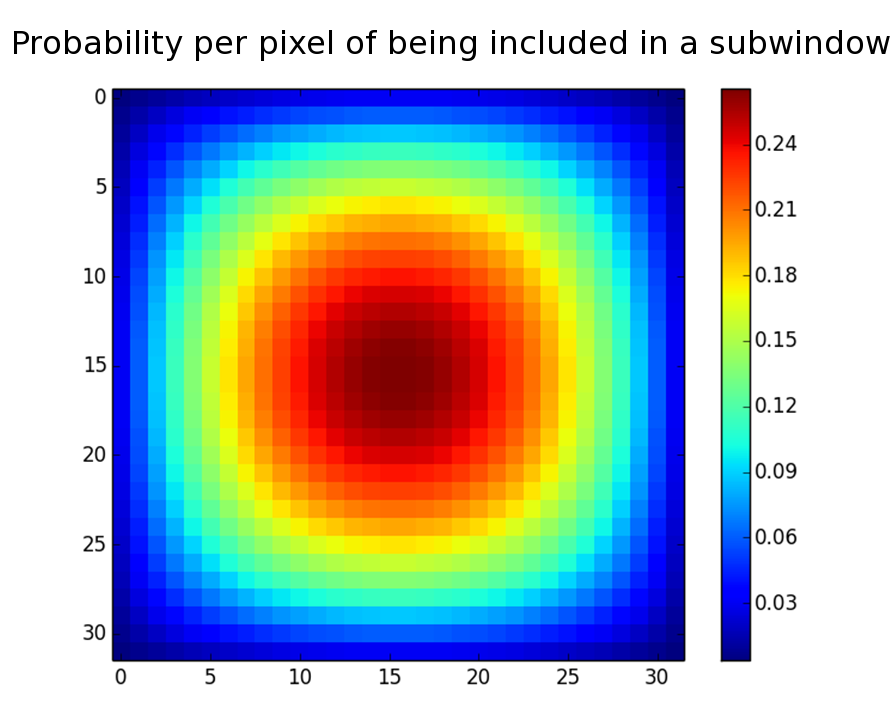
\includegraphics[width=0.6\textwidth]{images/probpixel.png}
		\caption{\label{fig:probpixel}Probability associated to each pixel of being picked up}
	\end{figure}
		
		\paragraph{}
		Although the subwindows can have different sizes, the feature vector describing a particular one cannot. More specifically, a column of the learning matrix must correspond to a well identified variable. Thus, we need to rescale all the subwindows to a common size. Ideally, the size should be chosen so as to minimize the re-interpolation deformation. The interpolation algorithms provided are nearest neighbor, bilinear and bicubic. We will focus on the nearest neighbor because it is faster and it was found to be comparable in term of classification accuracy to the others in most cases (\cite{base}).
		
		\subsection{Feature descriptions}		
		Each filtered and spatially pooled image will be described by its raw pixels in a last-dimension-first fashion. Therefore, we start by the color dimension and group the three color values of the top left pixel together. Then we append the second pixel (top row, second pixel from the left) and so on for all pixels of the first row. After that, we append the second line in the same fashion and so on for all the image. This is resumed by figure \ref{fig:imgDesc}, which also shows that the feature vectors belonging to the same subwindows are concatenated.
		Thus, there are $3(h \times w) \times (N \times P)$ features per subwindows. For instance, 100 filters with 1 pooling on 16x16 subwindows yields feature vectors of $3(16 \times 16) \times 100 = 76,800$ variables.
		
	\begin{figure}
		\centering
			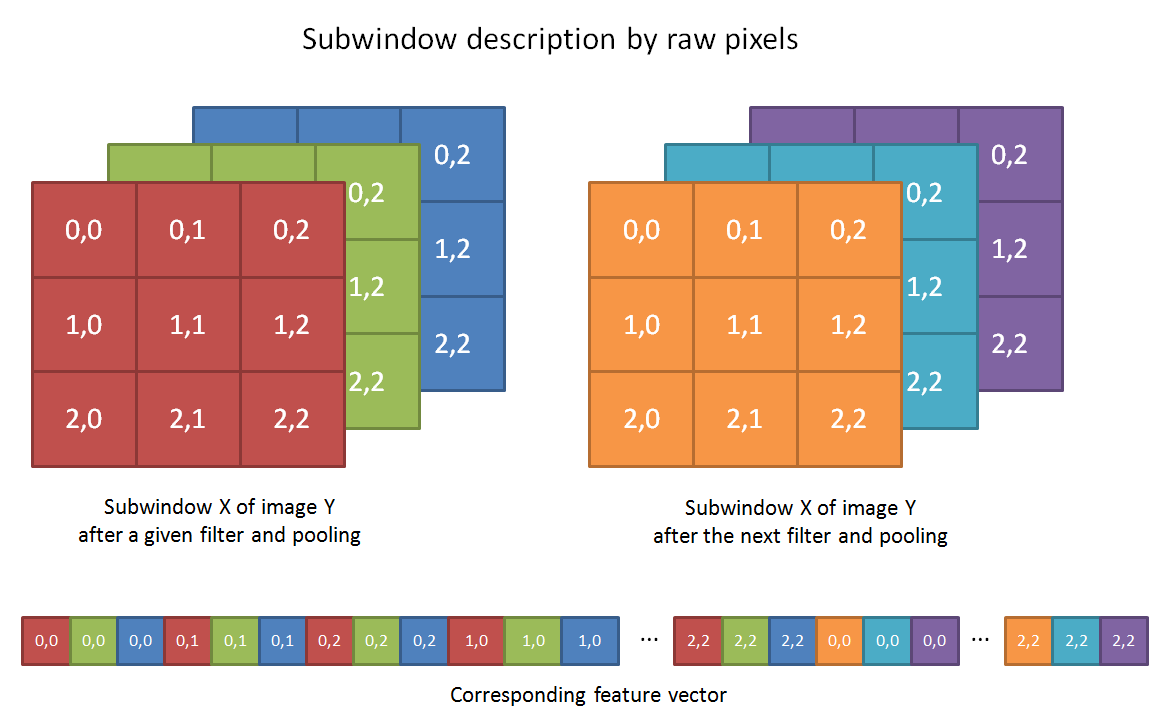
\includegraphics[width=1.0\textwidth]{images/imgDesc.png}
		\caption{\label{fig:imgDesc}Filtered and spatially pooled image description}
	\end{figure}
	
	\paragraph{}
	Once all the subwindows have been described in this fashion, we need to assemble each piece to form the actual learning matrix.
	Starting from the original database of $M$ images, a set of $N$ filters and $P$ spatial poolings, we produced $N \times P$ images for each original ones. From each of those $M$ sets, we extracted $S$ subwindows on each of the $N \times P$ filtered and pooled images. We now have $M \times S$ learning objects described by $N \times P$ feature vectors. As we mentioned earlier, we will concatenate all the feature vectors corresponding to the same subwindow. This is depicted by figure \ref{fig:LearningMatrix}.
	
	\begin{figure}
		\centering
			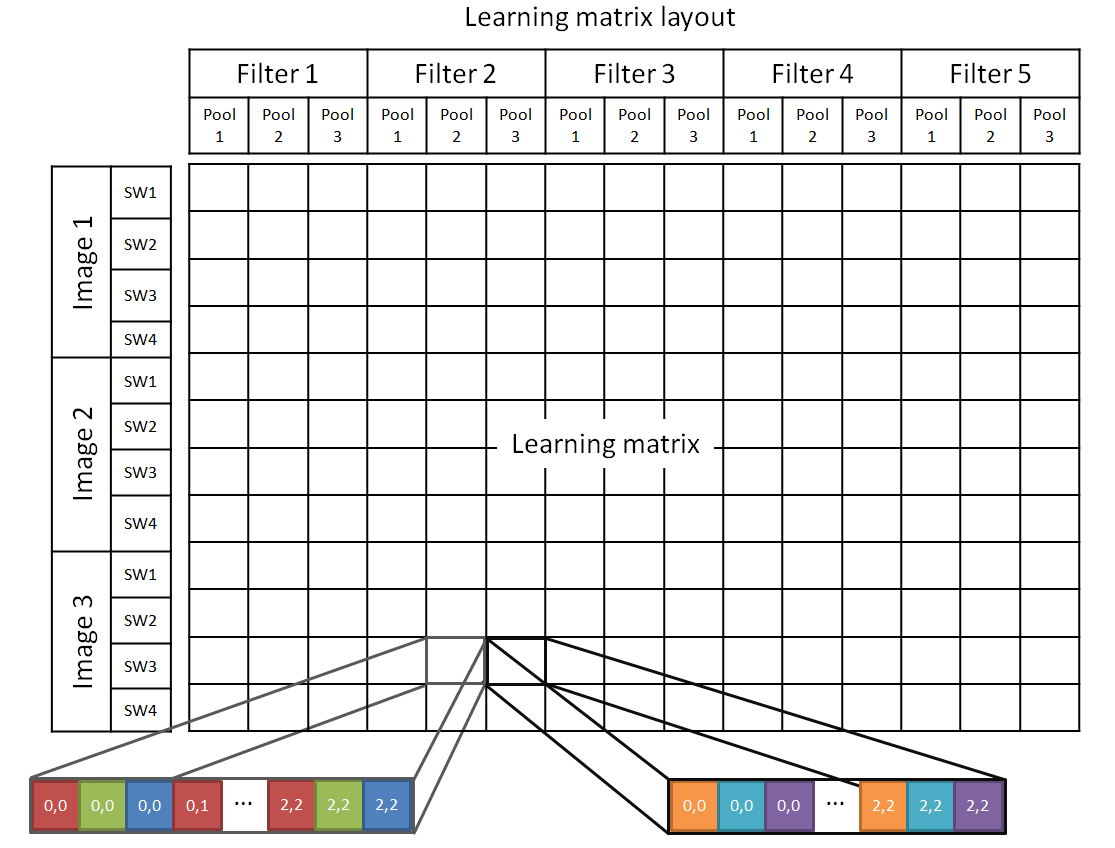
\includegraphics[width=1.0\textwidth]{images/LearningMatrix.png}
		\caption{\label{fig:LearningMatrix}Layout of the final learning matrix}
	\end{figure}	
		
		\subsection{Compression layer}
		An additional so-called compression layer was envisioned for two reasons. It works by reducing the number of features require to describe a subwindow. The first reason was to limit memory usage and the second one was to reduce the relative number of features associated to a given filter compare to the original image so as to put more emphasis on it.
		Two mechanisms were implemented. The first one is an additional layer in the feature descriptions part and only works on subsets of the  feature vectors. The second compression layer is situated after the traditional RandConv and works on the whole learning matrix.
		
		\paragraph{Feature subvector compression.}
		In this variant, we treat all the feature subvector separately. A subvector corresponds to the contiguous part of a subwindow feature vector related to one filter and pooling. The idea was to reduce the number of variables of such subvectors while losing as little information as possible. In order to accomplish that, we reduce the number of variable by selecting only one or two colors by pixel. The variables are chosen so that neighbor pixels of the same row have not the same color missing. In that way, we rely on spatial redundancy to limit the loss of information. This is illustrated by figure \ref{fig:imgDescCompression}. The compression rate is of $\frac{3}{2}$ for a low compression keeping two colors by pixel or $\frac{3}{1}$ for a high compression keeping only one color by pixel.
		Let us note that this variant does not allow for a separate treatment of the original image.
		
		\begin{figure}
		\begin{subfigure}{.5\textwidth}
			\centering
			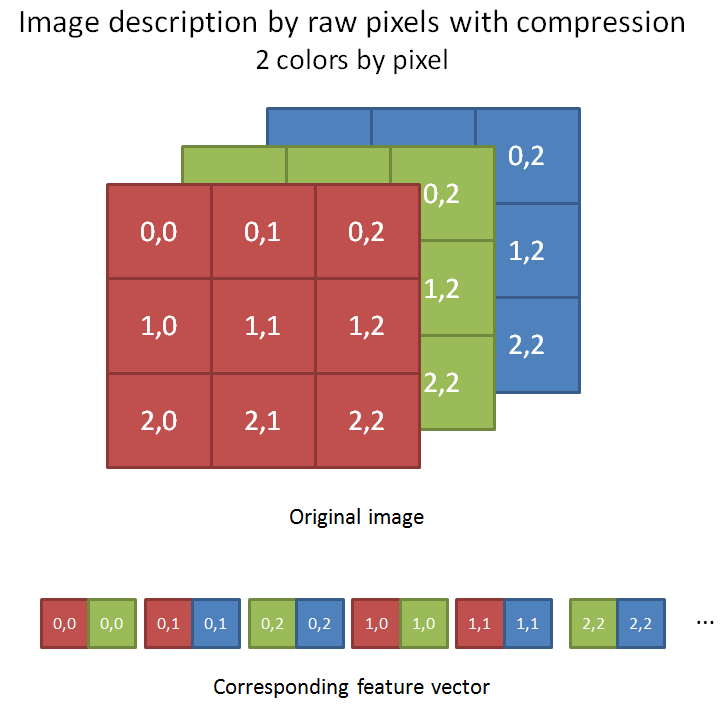
\includegraphics[width=1.\linewidth]{images/imgDesc2col.png}
			\caption{\label{fig:imgDesc2col}}
		\end{subfigure}%
		\begin{subfigure}{.5\textwidth}
			\centering
			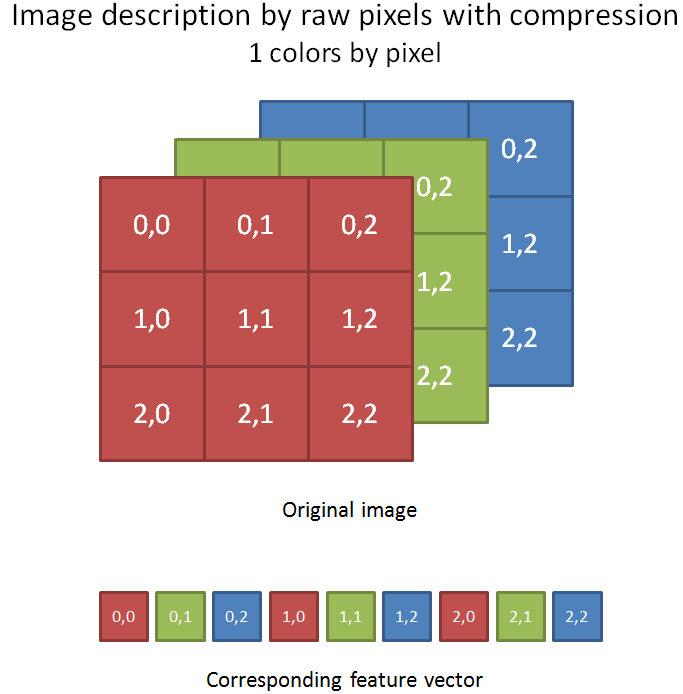
\includegraphics[width=1.\linewidth]{images/imgDesc1Col.png}
			\caption{\label{fig:imgDesc1Col}}
		\end{subfigure}
		\caption{\label{fig:imgDescCompression}Feature subvector compression}
	\end{figure}
		
		\paragraph{Learning matrix compression.}
		In this variant, we work on the whole learning matrix by reducing the number of variable associated to each combination of filter and pooling with the knowledge of all the learning objects. The method can treat the original image independently and the processing of the other group of features can be parallelized. Using the whole learning matrix allow for more sophisticated compression techniques, which can look for structure in the submatrices. This component works like a learning algorithm as well in the sense that it must fit itself on the learning matrix and then remember its choices for the prediction part.
		The layer is generic meaning that the processing can be parametrized.
		\par
		We implemented two such processings. The first one, was simply to draw randomly a subset of different features for each filter. The second one is a bit more elaborated and complex. It computes the principal component analysis (PCA) on all the features of a given filter and selects the first components. Therefore, the new features are linear combination of the original ones. In both cases, the compression rate can be tuned. 
		\par
		Although both mechanisms are unsupervised, it is possible to exploit the labels as well.
		
		\subsection{Classification schemes}
		The previous subsections cover the preprocessing steps to go from a database of images to an actual learning matrix. Now is the time to delve into the actual classification mechanism. We will use two approaches described in the following. 
		
			\subsubsection{Direct classification}
			In this ET-DIC (ExtraTrees for direct image classification) variant, the classification is undertaken by the ExtraTrees directly.
			Let us note that this scheme allows not only for individual feature importance evaluation but also for filter relevance evaluation by aggregating the importance of all the features corresponding to a given filter. This metric is surely a good candidate for filter co-usefulness evaluation.
			\paragraph{}
			The best results of the ET-DIC strategy in Pixit mode on the CIFAR-10 database was an accuracy rate of 53.67\% (\cite{base}). The corresponding hyper-parameters were the following : 10 fully grown trees, 20 subwindows of 75-100\% of the original size reshaped by nearest neighbor interpolation to 16x16 image described by raw pixel values and inspecting all the features on each node.
			
			
			\subsubsection{Feature learning scheme}
			In this ET-FL (ExtraTrees for feature learning) variant, the ExtraTrees are not used as classifier any longer but rather form a preprocessing step whose output will constitute the learning matrix of the actual classifier. It has been described in subsection \ref{subsec:BagOfVisualWord} about bag of visual words. The slight novelty is that ExtraTrees are used in an unsupervised way by selecting randomly the splitting criterion (including the splitting variable) of each node, a variant called totally randomized trees. Totally randomized trees as classifier usually perform less well than ExtraTrees (\cite{extratrees}). However, in the current context, the actual classification is delegated to a SVM. The gain of using totally randomized trees is computational.
		\par
		Since we are in the presence of more than two classes, we will resort to the one-versus-all scheme. It consists on training a SVM for each class. The ith model is learned by considering two classes : the ith original class on the one hand and all the other classes on the other hand. The prediction is carried out by assigning the class furthest from its margin. This is illustrated by figure \ref{fig:SVMOneVersusAll}
		\begin{figure}
			\centering
				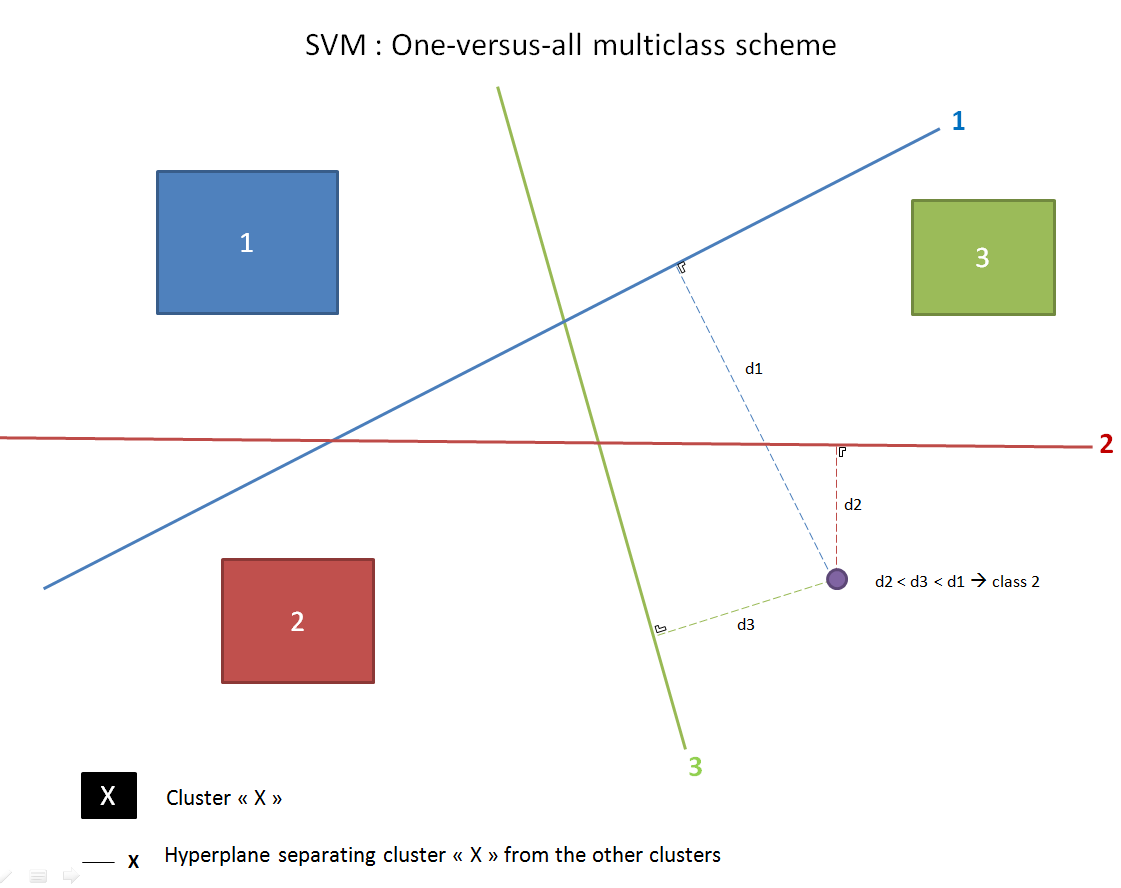
\includegraphics[width=0.7\textwidth]{images/SVMOneVersusAll.png}
			\caption{\label{fig:SVMOneVersusAll}One-versus-all multiclass scheme}
		\end{figure}
		
		\paragraph{}
		An important remark is in order, the learning size, and consequently the number of subwindows, is now crucially important. Indeed, it is one of the most influent parameters on the trees' depth, and consequently the number of leaves. 
		A second first-class parameter is the one relating to pruning. Pruning is the mechanism of stopping the tree creation before its completion. It can be applied either while developing the tree (pre-pruning) or artificially after the tree creation by cutting of some branches. It obviously also impact dearly the number of leaves. The main goal of pruning is to reduce the model complexity and consequently the overfitting. In the ET-DIC variant, pruning is not necessary because the voting takes care of reducing the overfitting. However, on the data fed to the SVM, there is no automatic overfitting control mechanism and the SVM will suffer from it. Therefore, pruning is also very important for this variant.
		Last but obviously not least, the number of trees multiply the number of leaves. Therefore, this hyper-parameter is even more sensitive than in the ET-DIC approach.
		
		\paragraph{}
		The best results of the ET-FL strategy in Pixit mode on the CIFAR-10 database was an accuracy of 50.07\% with 10 almost fully grown trees, 20 subwindows of 75-100\% of the original size reshaped in 16x16 by nearest interpolation and using $k = \sqrt{M}$ of inspecting features at each node, where $M$ is the total number of features : 16x16x3. The trees are not totally grown : the minimum number of samples to split a node is fix to 10. Contrary to the majority of cases, the best ET-DIC is better than the best ET-FL for this problem.
	\par
	Using the precursory method (equivalent to the custom filter generator) with 9 spatial poolings (3x3 to 7x7 moving windows computing the minimum, maximum and mean) they were able to obtain a significant raise of accuracy, attaining a new record of 74.31\% with 750 trees totally randomized trees, 20 subwindows and a minimum number of samples to split of 750 (\cite{base}).
			

	
	\section{Implementation}
	
	In this section, we dive into implementation details. We will not go over all the elements in depth again but rather see how the discussions of the previous sections translate into code. In a second subsection we will also develop technical limitations.
		\subsection{Software architecture}
		A major concern of the design was to allow as much room as possible for flexibility, so as to be able to develop extensions and variants of the method rapidly. Consequently, the code was split into many classes. A drawback of this is that assembling all the pieces together might be difficult. Factory methods are provided to help with this issue but care must be taken to build up a coherent classifier. We will go back on this in a short while. 
		\par
		The code is written in Python 2.7 and relies and the 0.13.3 version of Scipy (\cite{scipy}), including Numpy 1.8.0. Not all the code is brand new. The ExtraTrees implementation comes from the scikit-learn library (\cite{sklearn}), version 0.15. We also use scikit-learn for SVM classification, although it actually consists of a wrapper to the liblinear library (\cite{liblinear}). The SVM computes the optimal linear soft margin and manages multiclass by one-versus-all.
				As for the subwindow extraction, it is a reorganization of the Pixit implementation (\cite{cytomine}).
		We will examine the code in a top-down manner and focus on the important classes.
		\paragraph{}
		At the top, we find the \texttt{Classifier} class. Its aim is to supervise all the parts. The base class correspond to the ET-DIC variant. The \texttt{RandConvCoordinator} is responsible for all the preprocessing : filtering, pooling, subwindow extraction, feature description. After this step, the \texttt{Classifier} instance delegates the actual classification to a \texttt{BaseEstimator} instance from scikit-learn. In this case, the actual classifier is supposed to be an instance of \texttt{ExtraTreesClassifier}. The \texttt{UnsupervisedVisualBagClassifier} corresponds to ET-FL mode. Between the preprocessing and the classification, we use the \texttt{RandomTreesEmbedding}, a scikit-learn totally randomized trees implementation, to build the histogram which we will then fed to the \texttt{BaseEstimator}, supposed to be a \texttt{LinearSVC} instance.
		This is summarized by figure \ref{fig:uml-classifier}.
		
		
		\begin{figure}
			\centering
				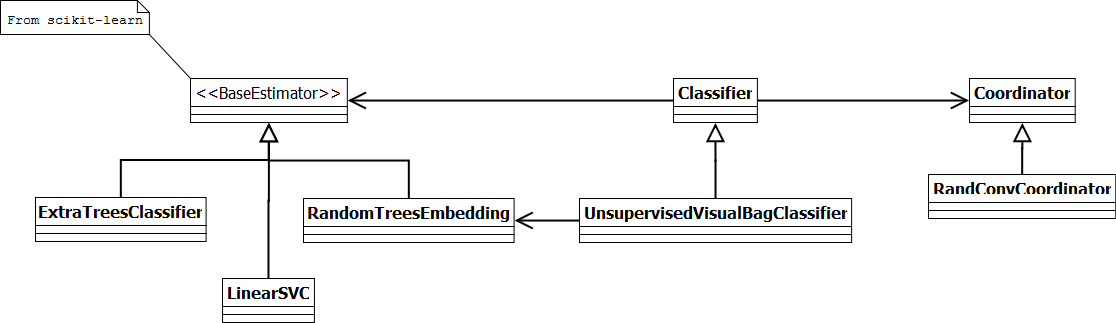
\includegraphics[width=1.00\textwidth]{images/uml-classifier.png}
			\caption{UML representation of the \texttt{Classifier} class and its major components}
			\label{fig:uml-classifier}
		\end{figure}
		
		
		\paragraph{}
		We now go back to the \texttt{RandConvCoordinator}. Its responsibility is to transform the image database into the learning matrix. It proceeds by subdividing the dataset to parallelize the transformation. Then, the \texttt{ConvolutionalExtractor} process each image. This entails filtering the image by each element of the \texttt{FiniteFilter} thanks to the \texttt{Convolver}, then applying all the spatial poolings contained in the \texttt{MultiPooler} and finally extracting several subwindows via the \texttt{MultiSWExtractor}. Once all this is done, each filtered and pooled subwindow is passed through the \texttt{Extractor} and reassembled to form a coherent learning submatrix.
		\par
		The \texttt{FiniteFilter} objects are containers for filters. They pre-generate a finite number of filters thanks to the \texttt{FilterGenerator}. We will come back to those shortly. If we are working with RGB images, we need to use either a \texttt{Finite3Filter} or a \texttt{Finite3SameFilter}. The former produces a different filter per color component while the latter uses the same filter on each color. Also, we need to use an appropriate \texttt{Convolver}, namely the \texttt{RGBConvolver}.
		\par
		The subwindow extraction is carried out by the \texttt{MultiSWExtractor} whose sole purpose is to keep track of the subwindows to extract for the set of filtered and pooled images belonging to the same original image. The actual subwindow generation and extraction are delegated to the \texttt{SubWindowExtractor}.
		\par
		The transformation from subwindows to feature vector is the responsibility of the \texttt{Extractor} instance. In this case, a \texttt{ImageLinearizationExtractor} object. However, other mechanism could be implemented, such as extracting descriptive statistics.
		All this is summarized by the figure \ref{fig:uml-ConvolutionalExtractor}. Let us note that the images are only loaded at the time they are processed so as not to drain useless memory. Python's garbage collector is responsible for freeing them as soon as needed after they were treated.
		
		
		\begin{figure}
			\centering
				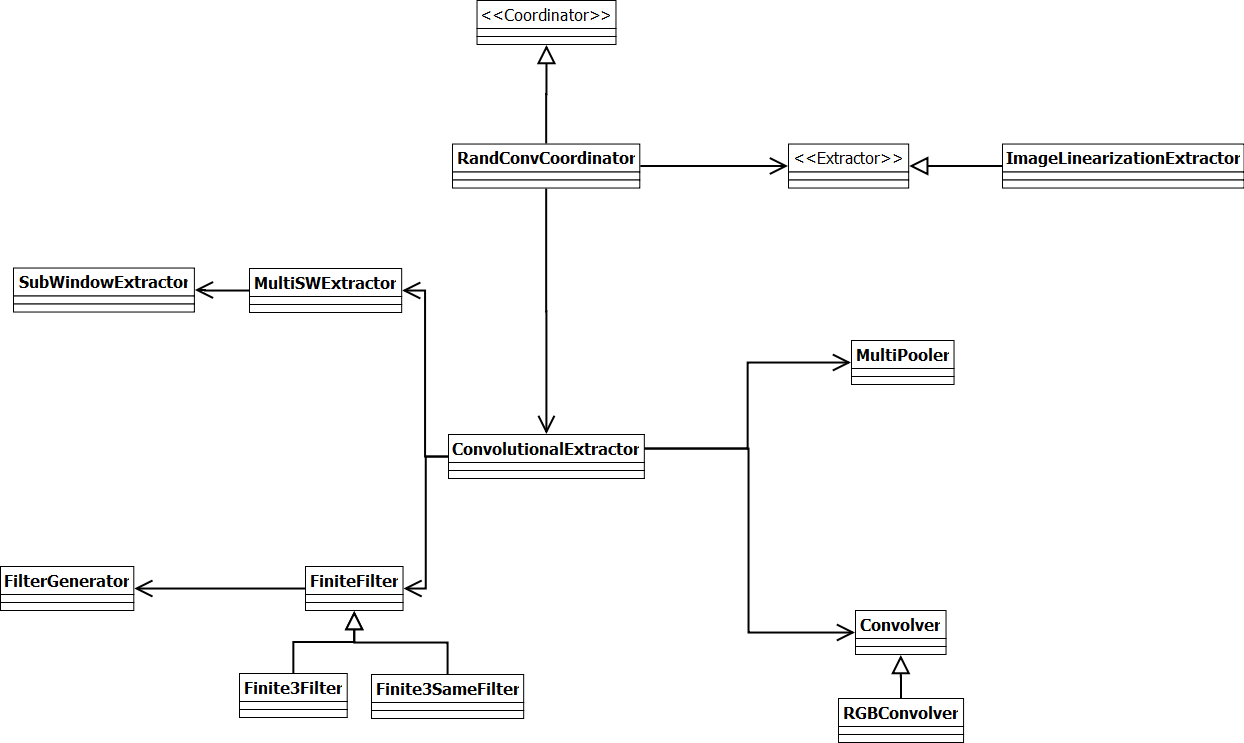
\includegraphics[width=1.00\textwidth]{images/uml-RandConvCoord.png}
			\caption{UML representation of the \texttt{RandConvCoordinator} and its major components}
			\label{fig:uml-ConvolutionalExtractor}
		\end{figure}
		

		
		
		\paragraph{}
		We now explore the \texttt{FilterGenerator}. They need two random number generators. One for drawing the values, either directly or not, and one for drawing the size. The base class is used for two of the generation methods : the discrete law generator and the zero-perturbation generator. The former is made by using a \texttt{CustomDiscreteNumberGenerator} while the later uses the base class of \texttt{NumberGenerator}. 
		As figure \ref{fig:uml-filtergen} displays, there is a class dedicated to each of the other generators.
		\par
		The \texttt{GaussianNumberGenerator} works by specifying a lower bound, an upper bound and the probability of being outside of that range. The \texttt{ClippedGaussianRNG} works similarly but in addition forces the values outside of the range to the appropriate bound.
		
		
		\begin{figure}
			\centering
				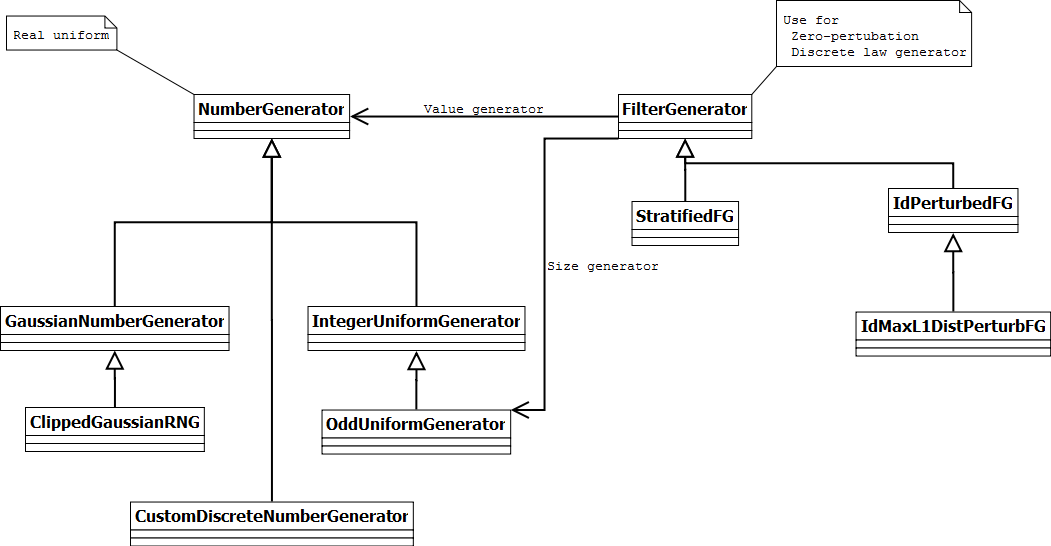
\includegraphics[width=1.00\textwidth]{images/uml-filtergen.png}
			\caption{UML representation of the \texttt{FilterGenerator}s and \texttt{NumberGenerator}s}
			\label{fig:uml-filtergen}
		\end{figure}
		
		
		\paragraph{}
		The \texttt{MultiPooler} class involved in the \texttt{RandConvCoordinator} is a container of spatial poolings. As the figure \ref{fig:uml-pooling} depicts, our two groups of spatial poolings are presents.
		\par
		Other classes are also present to take care of lesser chores, such as loading the data to the right format, logging the progress and so on.
		
		
		\begin{figure}
			\centering
				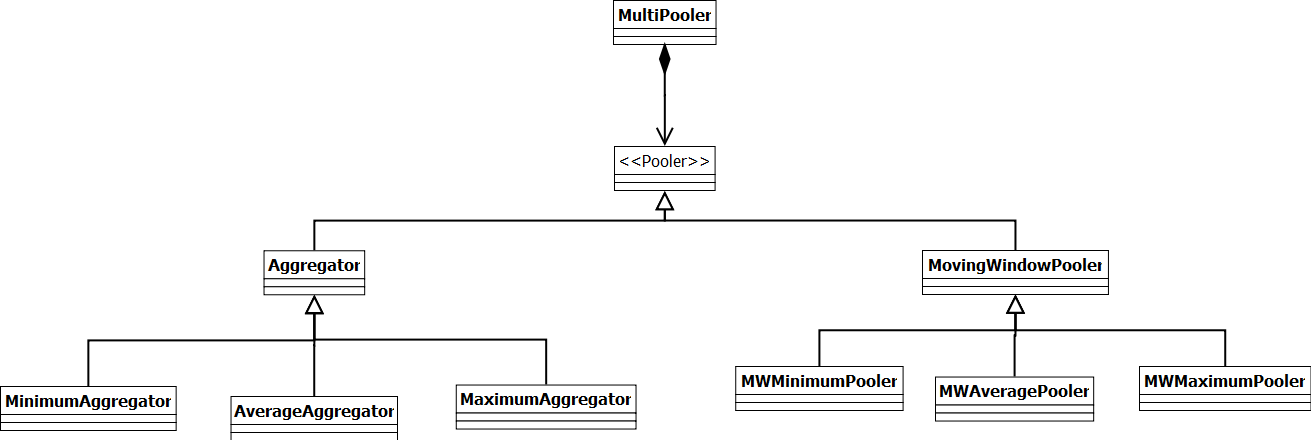
\includegraphics[width=1.00\textwidth]{images/uml-pooling.png}
			\caption{UML representaiton of the spatial poolings}
			\label{fig:uml-pooling}
		\end{figure}
			
		
		\subsection{\label{sub:TechnicalIssues}Technical issues}
		The main limitation we will face is memory. The ExtraTrees implementation require 32-bits floats and the SVM, 64-bits floats. However, in the case of the ET-FL, the matrix is mostly sparse on therefore the 64-bits floats requirement of the SVM will not be troublesome. Thus, the space cost bottleneck is the input of the ExtraTrees, which require to hold all the data in memory. Considering 100 filters, 1 spatial pooling, subwindows resized in 16x16, 3 colors, 10 subwindows and the whole learning set (50,000 images), the RandConv method will produce 153.6 GB of data. For 39 filters (the custom filters plus the original image) and 20 subwindows with 9 spatial poolings (the configuration of the best results of \cite{base}), 1,1 TB would be required. Since we are limited to 288 GB, we will not be able to reproduce such a configuration.
		\par
		One way of sidestepping this limitation is to build several forests with a different subset of the features, a variant which might be called ``global random subset'' (GRS) of features. 
		In the case of the RandConv this can easily be done by choosing a subset of filters for each forest.
		
		\paragraph{}
		To a lesser extent, the time complexity will be an hindrance. It will not actually prevent any computation but we will have to plan carefully the experiment to carry out. For instance, our first example, which produces 153.6 GB of data, takes between 5h and 12h depending on the machine load.
		
	\section{Hyper-parameters summary}
	Before elaborating on the results, we will rapidly summarize all the hyper-parameters involved with the RandConv framework.
	
	\begin{itemize}
	
		\item Filter generation
		\begin{itemize}
			\item Size range
			\item Whether or not to produce squared filters
			\item Value range
			\item Filter generator
			\item Random law
			\item Other filter generator specific parameters (maximum distance, number of subdivisions,...)
			\item Filter normalization
			\item whether or not to include the original image
		\end{itemize}
		
		\item Spatial poolings
		\begin{itemize}
			\item Number and type of poolings
			\begin{itemize}
				\item Aggregation or moving window
				\item Pooling function : identity, minimum, average or maximum
			\end{itemize}
			\item Size of the neighborhood
		\end{itemize}
		
		\item Subwindow extraction
		\begin{itemize}
			\item Number of subwindows
			\item Subwindows cropping size
			\item Subwindows rescaling size
			\item Subwindows rescaling interpolation
		\end{itemize}
		
		\item ExtraTrees
		\begin{itemize}
			\item Number of trees (default : 10)
			\item Number of features of the local random subspace : $k$ (default : square root of the total number of features)
			\item Maximum depth (default : no maximum depth)
			\item Minimum sample to split : $n_{min}$ (default : 2)
			\item Minimum sample per leaf (default: 1)
			\item Whether or not to use bootstrap (default : no bootstrap)
		\end{itemize}
	\end{itemize}
	
	As we can see, the number of hyper-parameters is already large. We can divide them in two categories. On the one hand, we have structural parameters and on the other, traditional hyper-parameters. Structural parameters have a more profound impact than traditional ones. The filter generator and its random law with the number and type of spatial poolings form the structural parameters. Conceptually at least, changing one of them is closer to changing the classification method than only one of its hyper-parameters.
	\paragraph{}
	Three of the ExtraTrees hyper-parameters are used to control the pruning : the maximum depth, the minimum sample split and the minimum sample per leaf. The difference between the last two is that the first one does not attempt to split a node whose number of samples are under the given threshold, while the second does the split but rollback if any of the children are under the threshold. 
	\paragraph{}
	Several of the parameters can be fixed. The value range of the filters will be set as in the filter generator descriptions. Considering the size of the images, we will mostly focus on 3x3 to 9x9 filters. Since we are working with trees, we will use no normalization of the filters. Concerning the spatial poolings, we will also restrict ourselves to small neighborhoods. For comparative purposes, we will resize subwindows to have sizes of 16x16 with nearest neighbor interpolation, as in \cite{base}. Moreover, we will extract subwindows of 24x24 to 32x32 pixels. For the ET-DIC variant, we will use the default trees parameters, which means no pruning. We will also use 30 trees (one per core). However, in the ET-FL approach, we will have to prune the trees and use more of them. The $n_{min}$ parameter will be set to 500 with 750 trees. Table \ref{tab:DefaultValuesForHyperParameters} displays the fix or default values of the hyper-parameters. Unless stated otherwise, these values are to be assumed in the next chapter.
	
	\begin{table}
		\centering
			\begin{tabular}{l|l}
			\hline
			Hyper-parameter & default value \\
			\hline
			Filter sizes & 3 to 9, both included\\
			Square sizes & True \\
			Filter value range & [-1, 1] \\
			Filter generator & \texttt{FilterGenerator} (Zero-perturbed generator)\\
			Random law & Real uniform\\
			Filter normalization & None\\
			Include original image & True\\
			Number of spatial poolings & 1 \\
			Type of spatial poolings & Average moving window \\
			Size of the neighborhood & 3x3 (moving window), 2x2 (aggregation)\\
			Number of subwindows & 10 \\
			Cropping size & 24x24 to 32x32 \\
			Rescaling size & 16x16 \\
			Interpolation & Nearest neighbor \\
			Number of trees & 30 (ET-DIC), 750 (ET-FL) \\
			$k$ & Square root of the total number of features \\
			Maximum depth & None \\
			Minimum sample to split & 2 (ET-DIC), 500 (ET-FL) \\
			Minimum sample per leaf & 1 \\
			Bootstrap & False \\
			\hline
			\end{tabular}
		\caption{Default values for hyper-parameters}
		\label{tab:DefaultValuesForHyperParameters}
	\end{table}
		


%================================================================================================================		
\chapter{\label{chap:results}Result analysis}
In this chapter, we describe the experiments conducted with our new classification method and analyze their results. The chapter is divided into two sections. The first one tackles the direct classification scheme (ET-DIC), where the forest of extremely randomized trees serves as classifier. The second section describes the other variant where the totally randomized trees are used to create a visual dictionary (ET-FL), while the actual classification is undergone by a support vector machine.
\par
When the hyper-parameters value are not explicit, the default values are to be assumed (table \ref{tab:DefaultValuesForHyperParameters} of page \pageref{tab:DefaultValuesForHyperParameters}).
%describe the succession of experiment
	\section{Direct classification scheme}
	
		\subsection{Accuracy as a function of the learning set size}
		Our first experiment will be to measure how the accuracies of the different methods evolve as a function of the learning set size. We will test the RandConv method with both types of pooling mechanisms (aggregation and moving window). The aggregation pooling uses a neighborhood of 2x2 while the moving windows are of size 3x3. Both poolings uses an averaging function. We will limit ourselves to the zero-perturbed filter generator for now. In both cases, the same 100 filter are drawn. The 10 extracted subwindows are resized to 16x16. Consequently there are $(16 \times 16 \times 100 \text{ filters} \times 1 \text{ pooling})\times 3 \text{ colors} = 76,800$ features. The accuracy is measured on the whole testing set composed of 10,000 images. The Pixit method will serve as reference. The RandConv method will be abbreviated by rci, for RandConv with original image.
		\paragraph{}
		We measured the accuracy for the learning set sizes of 500, 5,000, 10,000, 20,000, 30,000, 40,000 and 50,000. The result of this experiment is depicted by figure \ref{fig:accFLSsize}. The conclusion is clear : the aggregation pooling mechanism is not working (maximum of 0.38 of accuracy). Although being of the smallest interesting size, the non-overlapping neighborhood windows already lose too much of the information. One might argue that using 3x3 moving subwindows allow for that variant to capture more of the spatial structure than 2x2 neighborhood. However, this does not seem to be the case as using 3x3 neighborhoods yields a lower accuracy of 0.35 for the whole learning set. Therefore, the bad performances of the aggregation mechanism must indeed comes from its abusive spatial compression. This is unfortunate because those poolings suffered less from the rescaling of the extracted subwindows. Considering the gap of accuracy between both methods, the following experiments will focus on the moving window poolings.
		\par
		Other observations are worth mentioning. Firstly, the ``good'' RandConv method performs well. It is consistently better than the Pixit, although the difference might not be worth the trouble. The RandConv methods takes several hours whereas the Pixit requires a couple of minutes at most. 
		%Secondly, around 30,000 training images the accuracy rate slows down. This indicates that learning set is big enough to create models of the appropriate complexity.
		Secondly, the graph shows the impact of using only a subset of the data. This information is important in case of hyper-parameter optimization, for instance, where some of the data must be set aside as validation set.
		
		\begin{figure}
			\centering
				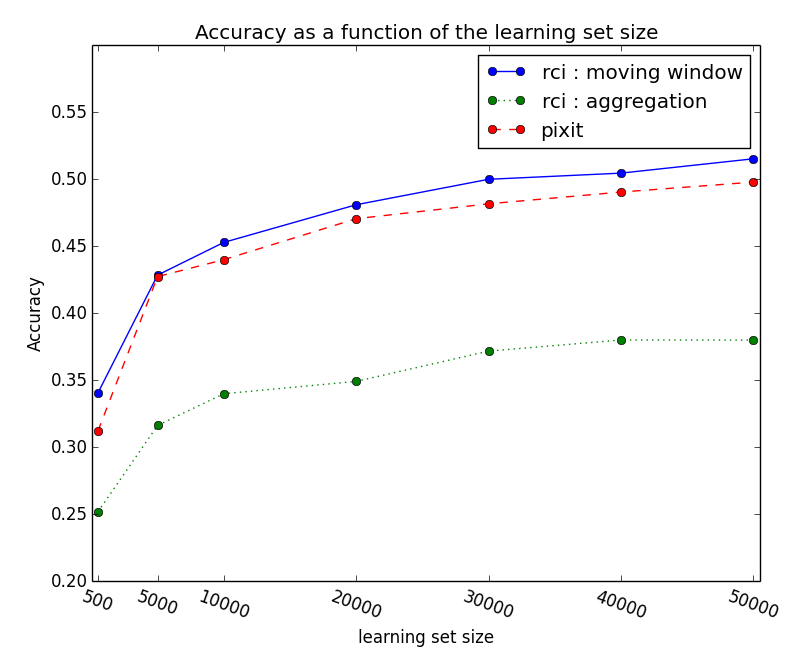
\includegraphics[width=1.0\textwidth]{images/accFLSsize.png}
			\caption{\label{fig:accFLSsize}Accuracy as a function of the learning set size (30 trees, $k=277$)}
		\end{figure}
		
		\paragraph{}
		Our best result so far is an accuracy of 0.5151 due to the RandConv method with moving windows for spatial pooling. The Pixit methods with the same parameters yields an accuracy of 0.50, while its best result is 0.5367 for 20 subwindows, 10 trees and a minimum sample to split of 10. We will now analyze the variability of the method and how the method reacts to some its hyper-parameters variations.
		%Validate small sized filters
		
		\subsection{\label{subsec:ETDICVariability}Variability}
		We now inspect the variability of the accuracy and of the filter importances. We will first look at the situation where the learning matrix is fixed and the variability can only come from the ExtraTrees. It is important to differentiate both types of variability. The one from the ExtraTrees would mainly be due to the high dimensionality of the problem. Indeed, the size of the local random subspace ($k = \sqrt{76,800} \simeq 277$) is relatively small compare to the total number of features : $\frac{277}{76,800} \simeq 3.6 \times 10^{-3}$. Therefore, different trees will end up making different choices. This is, of course, exactly the behavior we are looking for. However, with as few trees as 30, we may expect that different forests will have a high variability on the filter importances and consequently on the accuracy.
		
				\begin{table}
			\centering
			\begin{subtable}{0.5\textwidth}
				\begin{tabular}{c|c}
				\hline
				Test number & Accuracy \\
				\hline \hline
				0 & 0.5151 \\
				1 & 0.5119 \\
				2 & 0.5118 \\
				3 & 0.5136 \\
				4 & 0.5135 \\
				5 & 0.5141 \\
				6 & 0.5154 \\
				7 & 0.5114 \\
				8 & 0.5145 \\
				9 & 0.5156 \\
				10 & 0.5148 \\
				11 & 0.5118 \\
				\hline
				\end{tabular}
				\caption{\label{tab:AccVarTrees}Accuracy variability}
			\end{subtable}%
			\begin{subtable}{0.5\textwidth}
				\begin{tabular}{c|c}
				\hline
				Test number & Correlation with test 0\\
				\hline \hline
				0 & 1\\
				1 & 0.998 \\
				2 & 0.997 \\
				3 & 0.999 \\
				4 & 0.997 \\
				5 & 0.998 \\
				6 & 0.998 \\
				7 & 0.998 \\
				8 & 0.997 \\
				9 & 0.998 \\
				10 & 0.998 \\
				11 & 0.997 \\
				\hline
				\end{tabular}
				\caption{\label{tab:CorrMatFiltTreeVar}Correlation vector of the filter importances with test number 0}
			\end{subtable}
			\caption{\label{tab:TreeVar}Variability induced by the tree growing algorithm (same learning matrix)}
		\end{table}
		
		\begin{figure}
			\begin{subfigure}{.5\textwidth}
				\centering
				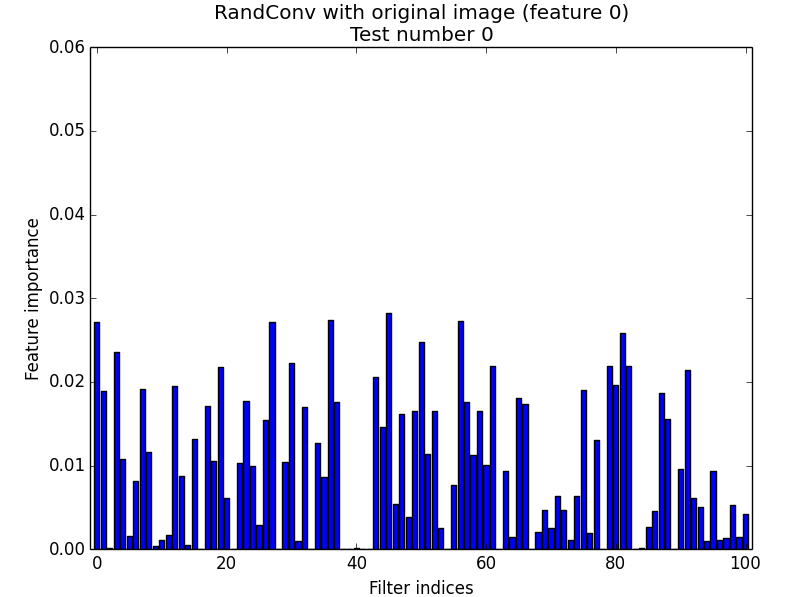
\includegraphics[width=1.\linewidth]{images/FIVarTree0.png}
				\caption{\label{fig:FIVarTree0}Test 0}
			\end{subfigure}%
			\begin{subfigure}{.5\textwidth}
				\centering
				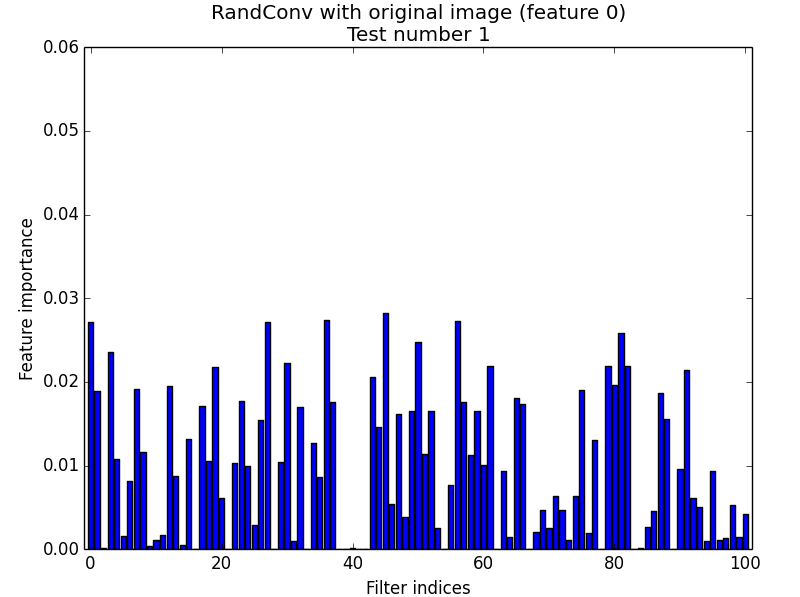
\includegraphics[width=1.\linewidth]{images/FIVarTree1.png}
				\caption{\label{fig:FIVarTree1}Test 1}
			\end{subfigure}
			\caption{\label{fig:FIVarTree}Filter importances for two different forests with the same parameters}			
		\end{figure}
		
		
		\paragraph{}
		We have run the ExtraTrees 12 times with the same hyper-parameters and the same learning matrix. Table \ref{tab:AccVarTrees} holds the accuracies and table \ref{tab:CorrMatFiltTreeVar} holds the first line of the correlation matrix of the filter importances between the tests. Figure \ref{fig:FIVarTree} depicts the filter importances for the two firsts tests. The test number 0 corresponds to the results given in the previous section. As we can see, the accuracy variability is very small. More tests would be needed to establish a rigorous confidence interval but the conclusion seems clear nonetheless : ExtraTrees variability has no impact on the accuracy. This is also backed up by the evident stability of the filter importances. Such stability is due to the smoothing effect of aggregating all the feature importances of a given filter.
		\par
		A look at the confusion matrices exposes more variability, notably on the diagonal. Despite the accuracy stability, the models are not exactly equivalent. This suggests that combining them or resorting to more trees will allow for some accuracy gain.
		\par
		Let us digress on the filter importances. From figure \ref{fig:FIVarTree}, we can see that several filters have a high importance ; of the same order of magnitude than the original image (filter 0). On the other hand, some filters bring little to no information in the classification process. Either these filters are not (co-)useful or the trees are too small to incorporate their usefulness. In regard to the correlations between tests, however, the co-usefulness and complexity hypotheses are less likely. If it were one of these problems, the low-rated filters would have developed on different trees and therefore the filter importance profiles would be less similar. Therefore, the most likely hypothesis is that those filters are simply not useful. Inspecting them in parallel of the best ones might reveal information about the classification task. In any case, removing them to make room for more interesting filters can only improve accuracy. Sadly, the gain might not be as substantial as we may hope. Indeed, the current accuracy gain compare to the Pixit is marginal, even though we already have many filters whose importance rivals the original image. 
		\par
		The overall conclusion is the following. For a given learning matrix, increasing the number of trees should not impact the filter importances because they are already quite stable. On the other hand, it should increase the accuracy because the models are not equivalent. The same conclusions should hold for the local random subspace size $k$, at least for the filter importances. In both cases, a decrease of the parameters may affect both the accuracy and filter profile. This variability analysis bring less insight to the minimum number of samples to split a node, $n_{min}$. Finally, as far as the accuracy and filter importances are concerned, the forest variability is negligible.

		\paragraph{}
		We now turn to the variability produced by the RandConv with the other parameters fixed to their default values. There are three sources of variability :
		
		\begin{itemize}
			\item The filter generated
			\item The subwindows extracted
			\item The trees built
		\end{itemize}
		
		As we have just seen, the last source of variability is negligible, therefore, we will mainly assess the first two ones. We ran 10 more tests whose accuracies are shown in table \ref{tab:VarZeropertAcc}. Test 0 corresponds to our previous test. Once again, more tests would be required to establish a proper confidence interval but the variability, although more important than previously, seems to be quite low. Tests number 0 and number 1 are particularly good. Nevertheless, this has to be put in perspective : such low range of accuracies, although always welcome for a practical application, is not really significant in our context.
		\par
		Since we are using different filters, the importance profiles will be different from one another. Figure \ref{fig:FIGVar} illustrates this for the tests number 1, 5, 6 and 10. We expect the ideal situation to be when all the filters have the roughly same importances. Nevertheless, how the filter importances influence the accuracy in other circumstances is unclear and cannot be determined from the importance profile. This is made clearer by comparing the cumulative importances of several tests. Figure \ref{fig:FIGVarCumHist} depicts the situation for tests number 0, 1 and 6. For the 30 most influential filters, test 6 is between the other two curves. After that point, test 6 depicts a greater cumulative filter importance. This situation also implies that there are more lowly important filter in test 6 than test 0 or 1. We cannot deduce anything from it because test 1 is also greater than test 0 in term of both the cumulative filter importance and accuracy. Besides, the cumulative profile of test 5 is nearly identical to the one of test 0. Therefore, it is impossible to assess finely the accuracy from the importance profile. This conclusion is also backed up by the areas under the curves.
		
		
		\begin{table}
			\centering
				\begin{tabular}{l|l}
				\hline
				Test number & Accuracy \\
				\hline \hline
				0 & 0.5151 \\
				1 & 0.5183 \\
				2 & 0.5117 \\
				3 & 0.5137 \\
				4 & 0.5095 \\
				5 & 0.5094 \\
				6 & 0.5093 \\
				7 & 0.5117 \\
				8 & 0.5129 \\
				9 & 0.5116 \\
				10 & 0.5124 \\
				\hline
				\end{tabular}
			\caption{\label{tab:VarZeropertAcc}Accuracy of several tests}
		\end{table}
		
		
		\begin{figure}
			\begin{subfigure}{.5\textwidth}
				\centering
				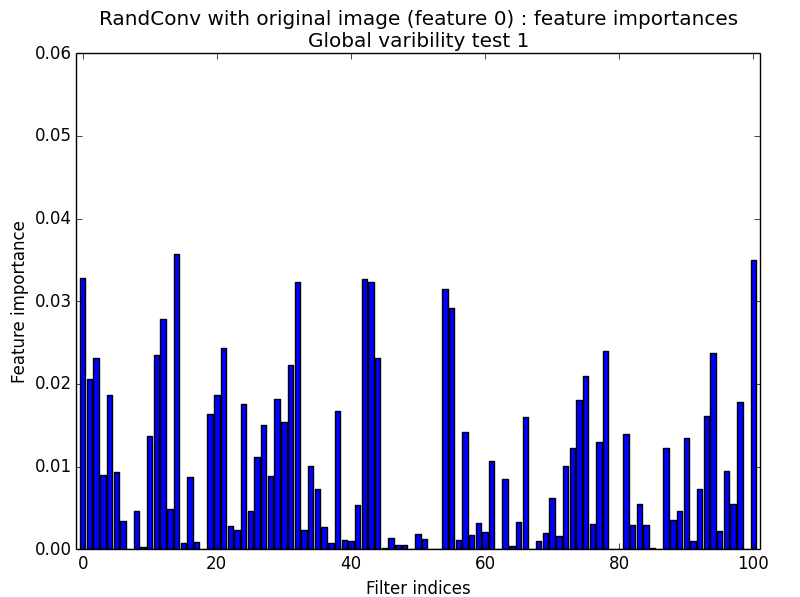
\includegraphics[width=1.\linewidth]{images/FIGVar1.png}
				\caption{\label{fig:FIGVar1}}
			\end{subfigure}%
			\begin{subfigure}{.5\textwidth}
				\centering
				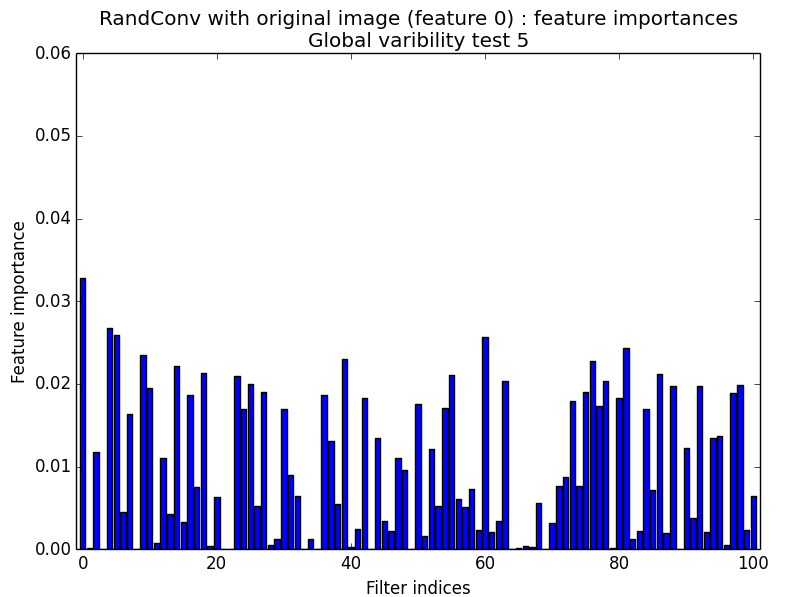
\includegraphics[width=1.\linewidth]{images/FIGVar5.png}
				\caption{\label{fig:FIGVar5}}
			\end{subfigure}
			\begin{subfigure}{.5\textwidth}
				\centering
				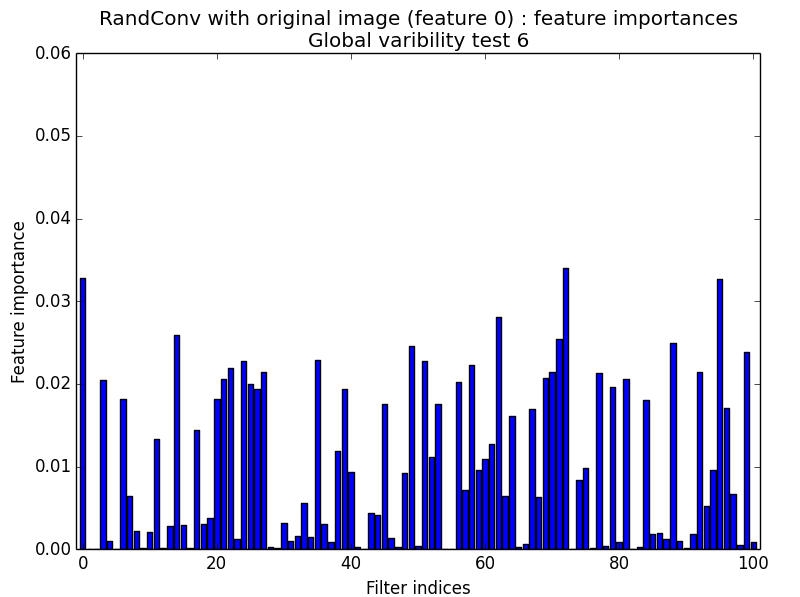
\includegraphics[width=1.\linewidth]{images/FIGVar6.png}
				\caption{\label{fig:FIGVar6}}
			\end{subfigure}%
			\begin{subfigure}{.5\textwidth}
				\centering
				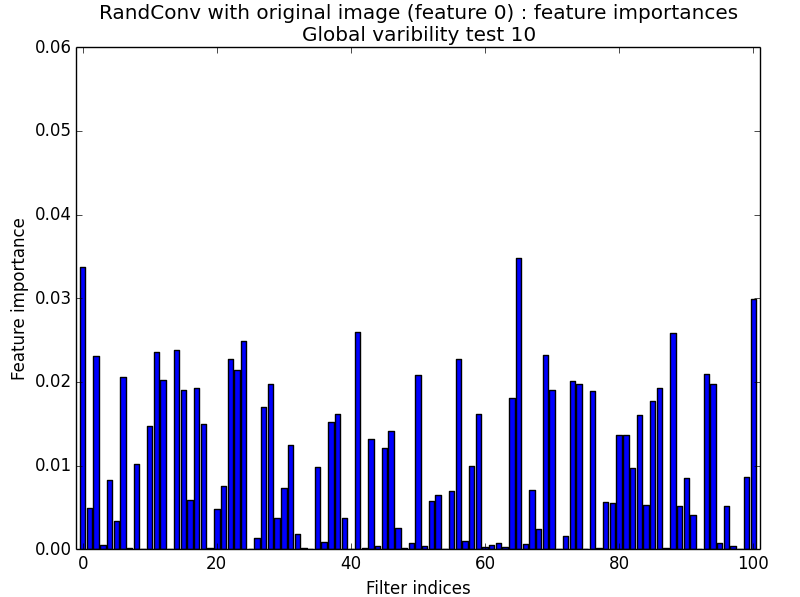
\includegraphics[width=1.\linewidth]{images/FIGVar10.png}
				\caption{\label{fig:FIGVar10}}
			\end{subfigure}
			\caption{\label{fig:FIGVar}Filter importances with global variability}
		\end{figure}
		
		\begin{figure}
			\centering
				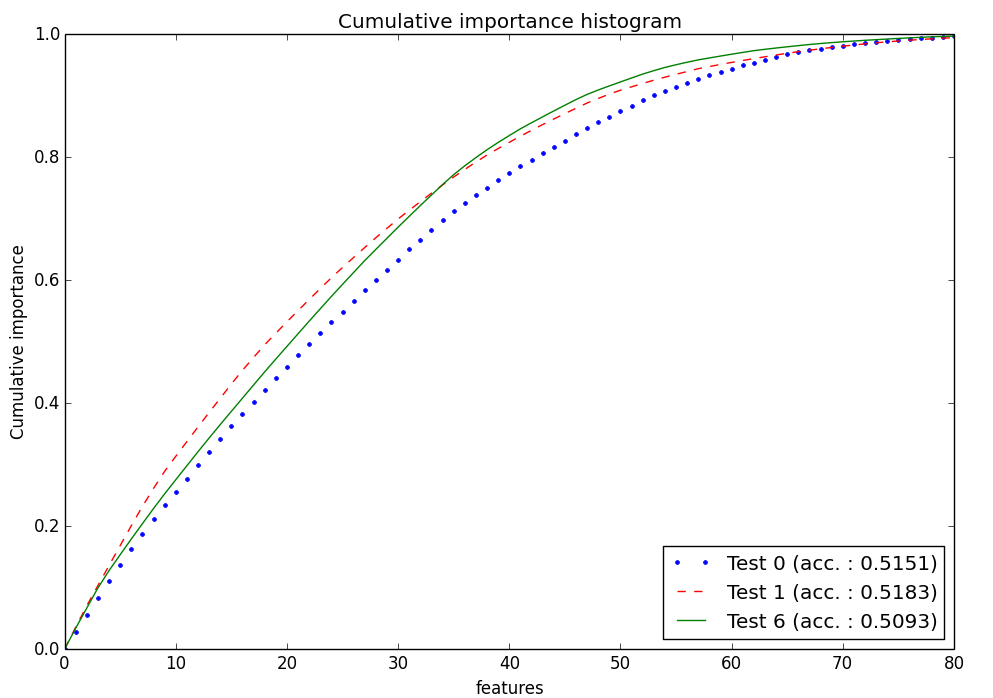
\includegraphics[width=1.0\textwidth]{images/FIGVarCumHist.png}
			\caption{\label{fig:FIGVarCumHist}Cumulative filter importance (first 80 filters)}
		\end{figure}
		
		\paragraph{}
		So far, we have learned that the RandConv method was surprisingly stable. Fortunately, this will allow us to draw conclusions from few experiments, a welcome surprise considering their running time. We will now inspect further the influence of hyper-parameters with a same set of filters if not a same learning matrix. We will roughly proceeds in a bottom-up fashion : starting from tree-related hyper-parameters and going to purely RandConv parameters.
		
		
		\subsection{Influence of the number of trees}
		\begin{figure}
			\centering
				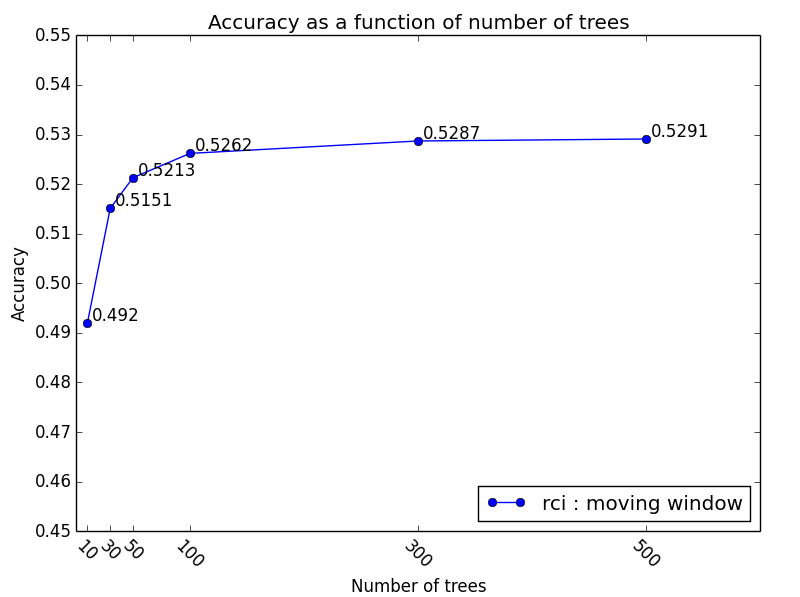
\includegraphics[width=1.0\textwidth]{images/accFnbTrees.png}
			\caption{\label{fig:accFnbTrees}Accuracy as a function of the number of trees}
		\end{figure}
		The accuracy is usually an increasing function of the number of trees. On the one hand, voting the prediction reduces model variability due to overfitting the data. On the other hand, each tree is unique and aggregating their prediction allow to encompass much more tests than what would be possible with a smaller forest. In this subsection, we will see how the improvement behaves for our method and we will look at the filter importances as well. In section \ref{subsec:ETDICVariability} about the variability, we foresaw that increasing the number of trees would have little influence on the filter importances. Now is the time to validate this thesis. Once again, the other parameters will be set to the default values of table \ref{tab:DefaultValuesForHyperParameters} on page \pageref{tab:DefaultValuesForHyperParameters} and the learning matrix is the same in all the tests. Consequently, the only source of variability is due to the forest creation.
		\paragraph{}
		In this experiment, we measure the accuracy for the following number of trees : 10, 30, 50, 100, 300 and 500. 
		The result of this experiment is depicted by figure \ref{fig:accFnbTrees}. As expected, we observe an increasing function of the number of trees. The increase slows down a bit at 100 trees with an accuracy of 0.526. After that, the increase rate drops considerably. Two remarks are in order. Firstly, we observe the classical increasing pattern, which means that the number of trees can be chosen solely with respect to the allowable computational budget. However, for a given learning matrix, the accuracy is upper bounded, as we can see from the rate decrease. Secondly, the 30-trees accuracy is closer to the 500-trees' than to the 10-trees'. Adding our observation about variability, we may conclude that using 30 trees allow us a good assessment of the method characteristics. 

		\par
		We now turn to the filter importances in the classification process. Table \ref{tab:CorrVecNbTrees} displays the filter importance correlation between the test with 10 trees and the other tests. As we had predicted, the number of trees does not impact the filter importances. Therefore, using 30 trees is well enough to assess filter usefulness as well.
		
		\begin{table}
			\centering
				\begin{tabular}{l|l}
				\hline
				Number of trees & Correlation \\
				\hline \hline
				10 & 1 \\
				30 & 0.996 \\
				50 & 0.998 \\
				100 & 0.998 \\
				300 & 0.998 \\
				500 & 0.998 \\
				\hline
				\end{tabular}
			\caption{\label{tab:CorrVecNbTrees}Filter importance correlation with 10 trees}
		\end{table}
		
		
		
		
		
		\subsection{Influence of local random subspace size}
		
		\begin{table}
			\centering
				\begin{tabular}{l|l}
				\hline
				Value of $k$ & Accuracy\\
				\hline \hline
				1 &  0.4467 \\
				50 & 0.4969 \\
				100 & 0.5057 \\
				277 & 0.5151 \\
				350 & 0.5172 \\
				500 & 0.5223 \\
				10,000 & 0.5276 \\
				\hline
				\end{tabular}
			\caption{\label{tab:AccFK}Influence of local random subspace size on the accuracy}
		\end{table}
		
		The parameter $k$ affects the individual tree variability and performances. Too low a value and trees are mostly random, ignoring the data at hand and consequently degrading accuracy. On the other hand, a high value might lead to a large redundancy between the trees, even though this is not the only randomization mechanism. Thus ending up with a lesser accuracy improvement from the forest's voting mechanism. 
		We ran the experiment using the following values of $k$ : $1$ (totally randomized trees), $50$, $100$, $277$ (the default value), $350$, $500$, $10,000$. The accuracies are presented at table \ref{tab:AccFK}. 
		As expected, the low values of $k$ decrease the accuracy. A value of $50$ does already quite well (closer to $10,000$ than $1$ in term of accuracy). It seems that going up to $10,000$ (13\% of the total number of features) does not yet reduces the accuracy. However, the increase may not be worth the time required to get it (more than twelve hours). Once again, the default value allows for capturing the essence of the method.
		\par
		The interesting part on the filter importances is that the profile correlation between the totally randomized trees and the default forest is still very high : 0.977. Therefore, it really means that the importances reflect the  filter usefulnesses.
		
		
		
		
		
		
		
		\subsection{Influence of the minimum number of samples to split}
		This parameter control the model complexity. In the previous experiments, the trees were fully grown ($n_{min} = 2$) and variability reduction was achieve through the smoothing effect of the forests prediction aggregation. Still, the model might be too complex to begin with, thus requiring either some pruning or more trees. Adding more trees did improve the model accuracy but, considering this has several impacts, we do not yet know whether we produce too complex models. So as to dissipate doubts, we tested the following values for this hyper-parameter : 2, 10, 50, 500. The corresponding accuracies are : 0.515, 0.512, 0.498, 0.453. Once again we see that the default value performs well. Besides, pruning too much the trees is harmful : the models are not complex enough any longer.
		
	\begin{figure}
		\begin{subfigure}{.5\textwidth}
			\centering
			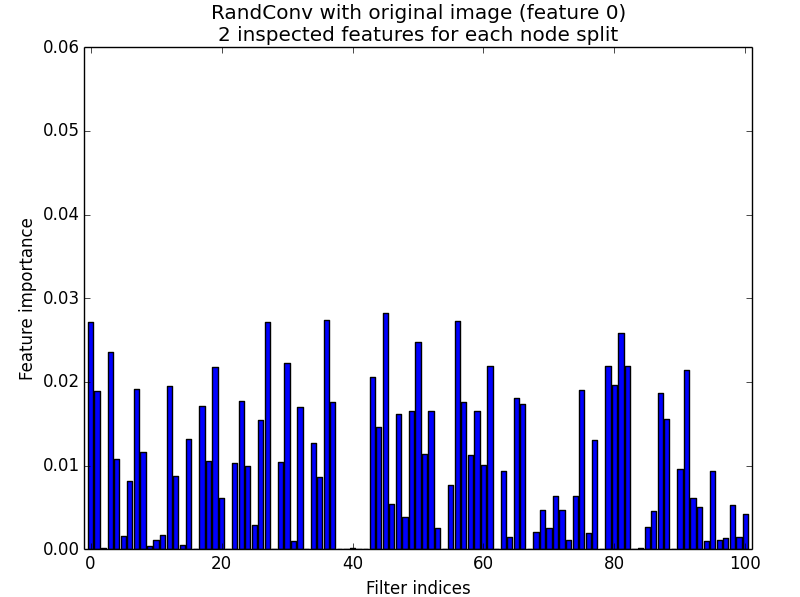
\includegraphics[width=1.\linewidth]{images/FInmin2.png}
			\caption{\label{fig:FInmin2}}
		\end{subfigure}%
		\begin{subfigure}{.5\textwidth}
			\centering
			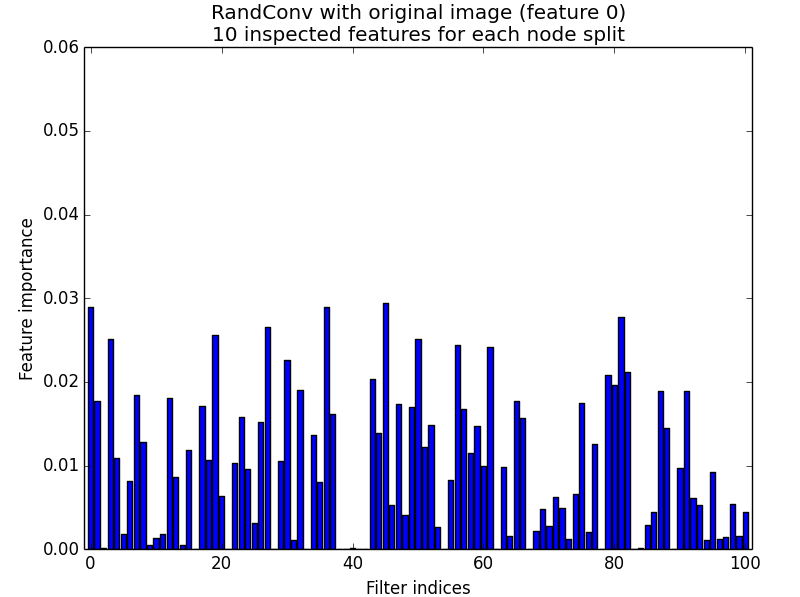
\includegraphics[width=1.\linewidth]{images/FInmin10.png}
			\caption{\label{fig:FInmin10}}
		\end{subfigure}
		\begin{subfigure}{.5\textwidth}
			\centering
			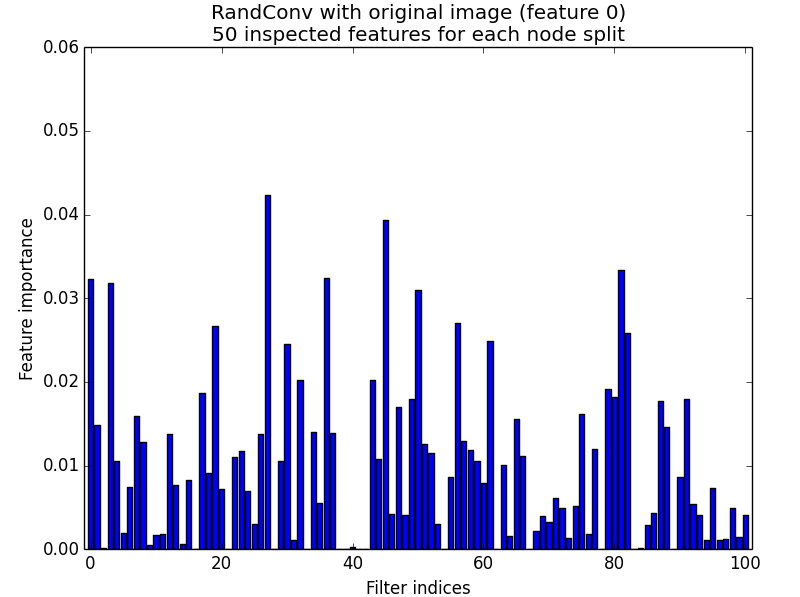
\includegraphics[width=1.\linewidth]{images/FInmin50.png}
			\caption{\label{fig:FInmin50}}
		\end{subfigure}%
		\begin{subfigure}{.5\textwidth}
			\centering
			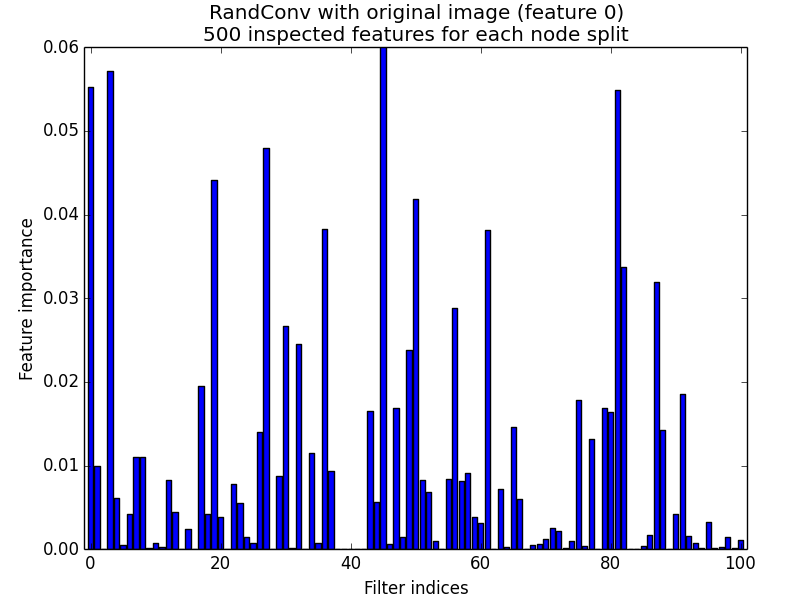
\includegraphics[width=1.\linewidth]{images/FInmin500.png}
			\caption{\label{fig:FInmin500}}
		\end{subfigure}
		\caption{\label{fig:FIPnmin}Filter importances for different values of $n_{min}$}
	\end{figure}
	
	
		\par
		The influence on the filter importances is more interesting. From figure \ref{fig:FIPnmin}, we clearly can identify two groups of filters. The first one is composed of the filters whose importance increases. This increase implies a decrease of the filter importances in the second group. It is thus possible to see where the filter is used in the trees. The first group holds the top of the tree. This was already obvious for the filters whose importance was either large or low. However, this approach sheds more light on the average filters, where we can observe divergent behaviors. Average filters of the second group are purely co-useful filters : they bring little information on their own but are helpful with the other filters. This characteristic resembles the ``V-structures'' of the graphical probabilistic models. On a specific classification task, these particular filters may be worth investigating. It might be difficult to identify the filters on which they depend, however.
	
		
		
		
		
		
	
		\subsection{Influence of the number of subwindows}
		As a reminder, the number of subwindows enlarges the learning set and therefore allows for more complex models. In this experiment, we tested how accuracy varied with the number of extracted subwindows. We used 1, 5, 10, 14 and 18 subwindows. The memory limited us to that threshold in order to keep the other parameters to their default values (table \ref{tab:DefaultValuesForHyperParameters}, page \pageref{tab:DefaultValuesForHyperParameters}). We also tested the method where no subwindows are extracted but rather the whole image is used directly. The results are reported at table \ref{tab:AccFNbSW}. The filters were the same in all the tests.
		\par
		As we might have suspected, using the whole image yields better accuracy than using only one random subwindows. However, a few of them already accounts for a better accuracy. Judging by the accuracy jump between 5 and 10 subwindows compare to the stagnation between 10 and 14 subwindows, we may conclude that 10 subwindows allows for complex-enough models. 
		
		\begin{table}
			\centering
				\begin{tabular}{l|l}
				\hline
				Number of subwindows & Accuracy \\
				\hline \hline
				1 (whole image) & 0.44\\
				1 (subwindow) & 0.40 \\
				5 & 0.48 \\
				10 & 0.515 \\
				14 &  0.514\\
				18 &  0.521 \\
				\hline
				
				\end{tabular}
			\caption{\label{tab:AccFNbSW}Accuracy as a function of the number of subwindows}
		\end{table}
		
		
	\par
	Once again, the filter importances correlation is high. In particular, it is above 0.997 between 5 and 10 subwindows.
	
		
		
	\subsection{Influence of the number of filters}
	Our expectation regarding the number of filters is that, with few of them, the accuracy might be better or worse than the Pixit's depending on the filter usefulnesses. Too many useless filters would hinder the process. With many filters, however, there should be enough usefulness altogether to be able to beat the Pixit systematically. The accuracy should increase accordingly with the number of filters as long as the learning set size allows for complex-enough model. However, from the comment on the variability (subsection \ref{subsec:ETDICVariability}), we suspect that we will reach an upper bound quite fast. 
	\par
	From a more practical point of view, we will have to limit ourselves to 180 filters, which should not be a problem if we were right about the upper bound. Table \ref{tab:AccFNbFilt} presents the accuracies for 10, 38 (the number of filters in the custom generator), 100, 120, 180 filters. As we can see, from 100 filters on, there is no accuracy gain and the filter and subwindow variabilities are responsible for the slight differences of accuracy. We would need a more profound analysis to determine whether or not the accuracy obtained with 38 filters is statically inferior to the 100 filter case's. In any case, it is closer to the accuracy of the 100 filters than of the 10 filters.
	
	\begin{table}
		\centering
			\begin{tabular}{l|l}
			\hline
			Number of filters & Accuracy \\
			\hline \hline
			10  & 0.4831 \\
			38 & 0.5087 \\
			100 & 0.5151 \\
			120 & 0.5112 \\
			180 & 0.5150 \\
			\hline
			\end{tabular}
		\caption{\label{tab:AccFNbFilt}Influence of the number of filters on the accuracy}
	\end{table}
	
	
	\subsection{Influence of the filter sizes}
	So far, we restricted the filter sizes to the range 3x3-9x9, implicitly focusing on local characteristics. The idea behind this was that larger filter would incorporate too global information and thus produce more useless redundancy. Besides this, larger filter also means more boundary problems. Nevertheless, the best sizes are problem and image sizes dependent. 
	We ran an experiment where we used sizes ranging from 3x3 to 31x31, while other parameters are left to their default value. The accuracy was of 0.4996, slightly less than for the standard case but not small enough to conclude much from it. Inspecting the feature importances brought more insight to the situation. Figure \ref{fig:FIBigFilters} depicts the situation. As we can see, the situation is more contrasted than usual. Linking the importances to  the sizes, we see that, in the top ten filter importance-wise, all 3x3 filters are present and the remaining three are 5x5. Furthermore, the other five 5x5 filters are in the top twenty, with 7x7 and 9x9 filters, mostly.
	
	\begin{figure}
		\centering
			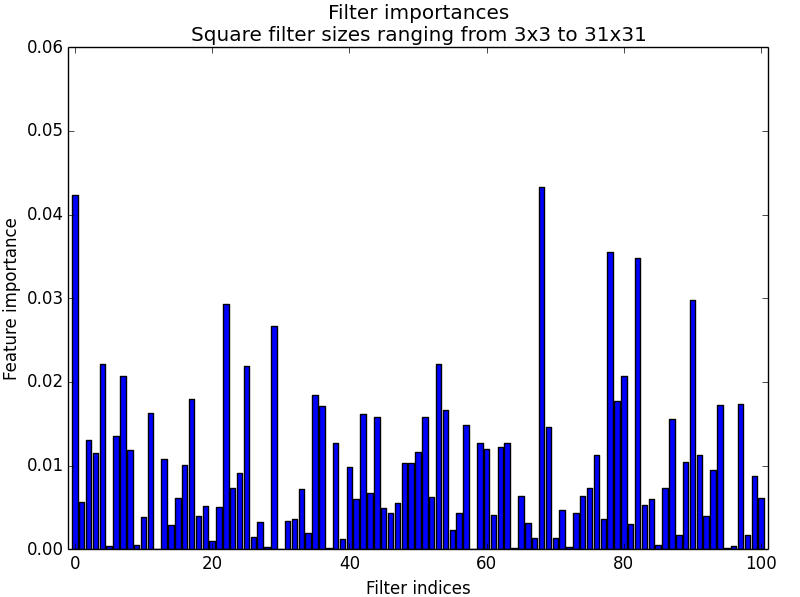
\includegraphics[width=1.0\textwidth]{images/FIBigFilters.png}
		\caption{\label{fig:FIBigFilters}Filter importances for filter sizes ranging from 3x3 to 31x31}
	\end{figure}
	
	
	
		
	\subsection{Influence of the filter generator}
	%Compare rci to rc
	In this section, we analyze the influence of the filter generator. We ran our experiments with the defaults values (table \ref{tab:DefaultValuesForHyperParameters}, page \pageref{tab:DefaultValuesForHyperParameters}), except for the parameters linked to the filter generators. We made the following experiments : 
	
	\begin{itemize}
		\item Custom filters (accuracy : 0.5057)
		\begin{itemize}
			\item Only 38 filters + the original image
		\end{itemize}
		\item Zero-perturbed generator with a discrete random law (accuracy : 0.509) :
		\begin{itemize}
			\item -1 with a probability of 0.3
			\item 0 with a probability of 0.4
			\item 1 with a probability of 0.3
		\end{itemize}
		\item Identity-perturbed generator with a real uniform law on $[-1, 1]$ (accuracies : 0.5085 and 	0.5154)
		\item Identity-perturbed generator with a Gaussian law of 0 mean and 0.51 standard deviation (accuracies : 0.5149 and 0.5135)
		\item Identity-perturbed generator with a Gaussian law of 0 mean and 0.36 standard deviation (accuracies : 0.5151 and 0.5119)
		\item Identity-distance generator with a maximum distance of 5 and a real uniform law (accuracies : 0.5068 and 0.5029)
		\item Identity-distance generator with a maximum distance of 10 and a real uniform law (accuracy : 0.4999)
		\item Identity-distance generator with a maximum distance of 5 and a Gaussian law of 0 mean and a probability of being outside of the range $[-maxDist, maxDist]$ of 0.005 (accuracies : 0.5032 and 0.5116)
		\item Identity-distance generator with a maximum distance of 10 and a Gaussian law of 0 mean and a probability of being outside of the range $[-maxDist, maxDist]$ of 0.005 (accuracies : 0.5049 and 0.5079)
		\item Stratified generator with a subdivision in 10 cells and a Gaussian law of 0 mean and 0.021 standard deviation (accuracies : 0.5088 and 0.5063)
		\item Stratified generator with a subdivision in 10 cells and a Gaussian law of 0 mean and 0.036 standard deviation (accuracy : 0.5109)
	\end{itemize}
	
	The standard deviation value of 0.51 is chosen so that the generated values have a probability of being outside the range $[-1, 1]$ of 0.05. The value of 0.36 reduces this probability to 0.005. As for the value of 0.021 and 0.036, they were chosen so that there is only a probability of 0.001 or 0.05, respectively, to be outside the range $[-0.07, 0.07]$. Let us remember that, in the case of the identity-distance generator, the drawing interval is not constant but decreases after each draw.
	
	\begin{figure}
		\begin{subfigure}{.5\textwidth}
			\centering
			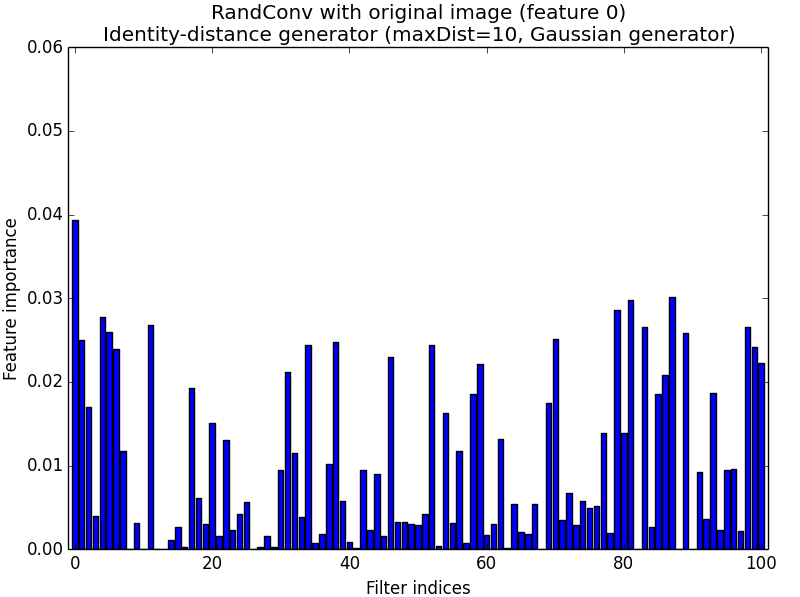
\includegraphics[width=1.\linewidth]{images/FIIdDistGauss.png}
			\caption{\label{fig:FIIdDistGauss}Maximum distance of 10 and Gaussian law}
		\end{subfigure}%
		\begin{subfigure}{.5\textwidth}
			\centering
			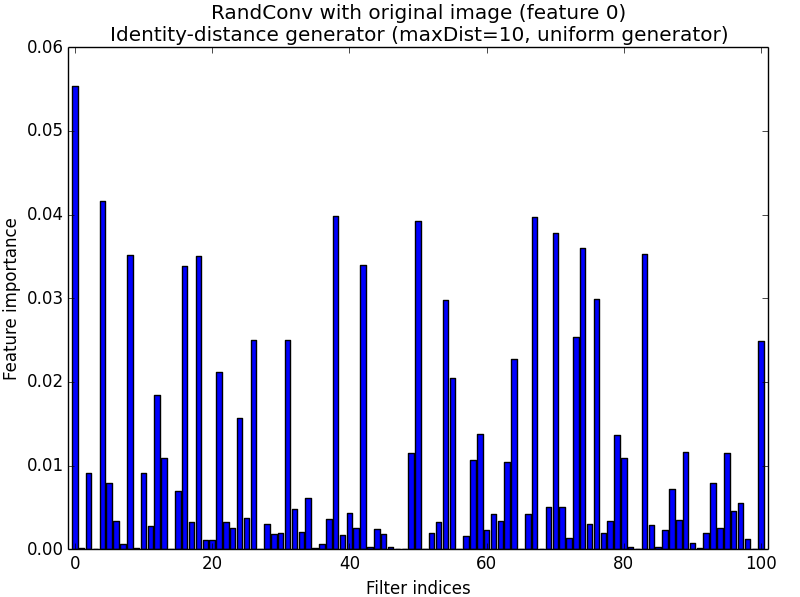
\includegraphics[width=1.\linewidth]{images/FIIdDistRU.png}
			\caption{\label{fig:FIIdDistRU}Maximum distance of 10 and real uniform law}
		\end{subfigure}
		\caption{\label{fig:FIIdDist}Filter importances of the identity-distance generators}
	\end{figure}
	
	\paragraph{}
	Judging from those experiments, we can see that identity-distance generator do worse than our usual generator. This is also visible from the filter profiles (figure \ref{fig:FIIdDist}), where we can see much more variability than what we were accustomed to.
	Considering the variability we have observed previously, the situation is unclear for the other generators, although the identity-perturbed suites tends to do well. In any case, the filter generator is not the most influential parameter. This is an important, disturbing and revealing result. Our initial expectation laid in the opposite direction : the filter generators were the cornerstone of the method. A good choice (or combination) of generators producing many filters should have helped unveil useful information for the classification. Sadly, this did not turn out as expected. Our last hope to get significant accuracy improvements now resides in the non-linear layer of spatial pooling.
	The bright side is that we do not have to worry much about optimizing those parameters ; the zero-perturbed or identity-perturb generators will do just fine.
	
	
	\subsection{Influence of spatial poolings}
	In this subsection, we tackle the influence of the spatial poolings with a couple of experiments. We will resort to the 39 custom filters so as to be able to use several poolings (the original image and the actual 38 filters). The only meaningful source of randomness is the drawing of subwindows. We tested the following scenarios : 
	
	\begin{itemize}
		\item No pooling (accuracy : 0.4816)
		\item 1 pooling : 3x3 moving windows assigning the minimum (accuracy : 0.5151)
		\item 1 pooling : 3x3 moving windows assigning the mean (accuracy : 0.5057)
		\item 1 pooling : 3x3 moving windows assigning the maximum(accuracy : 0.5476)
		\item 3 poolings : 3x3 moving windows assigning the minimum, the mean and the maximum respectively (accuracy : 0.5454)
		\item 3 poolings : 3x3, 5x5, 7x7 moving windows assigning the minimum (accuracy : 0.5294)
		\item 3 poolings : 3x3, 5x5, 7x7 moving windows assigning the mean (accuracy : 0.5173)
		\item 3 poolings : 3x3, 5x5, 7x7 moving windows assigning the maximum (accuracy : 0.5741)
		\item 1 pooling : 7x7 moving windows assigning the maximum (accuracy : 0.5675)
	\end{itemize}
	We can clearly see that the poolings have a beneficial effect on the accuracy, in particular the maximum. %test with maximal pooling on zeropert
	%rci_zeropert_120_filters no poolings : 0.4912
	Choosing the best pooling must either be done by cross-validation or not done at all : using several poolings should not reduce the accuracy dramatically. The main drawback of this last option is that the memory might be better used in another fashion. Using the same pooling at different spatial scales may or may not be interesting.

	
	\paragraph{}
	We now turn to the filter importances. Figure \ref{fig:FIPool} depicts the profiles for the single pooling cases. Some filters always have a high or low importance. For other filters, however, the importances vary. Concerning the profiles, if not the accuracies, the no pooling and average strategies are close, with a correlation of 0.954 (see the correlation matrix on table \ref{tab:FIPoolCorr}). The major difference comes from the number 20, which is a high pass filter. %Have a look at frequency response with and without the averaging
	The other pieces of information given by the correlation matrix are as one might expect.
	More interesting, we can observe that the profiles can be importantly influenced by the pooling, which means that it does bring information and increase some filter usefulnesses. In the occasion of filter 28 (the west compass gradient mask), the maximum pooling even goes as far as giving it more importance than other filters appreciated by the remaining poolings. 
	Interpreting the cumulative importance diagram (figure \ref{fig:FIPool}) is, once more, complicated and we will limit ourselves to the following observation. The maximum pooling is the closet example to a straight line (the ideal situation where every filter has the same importance) we have seen so far and also scores the best accuracy for now. Despite the closeness, the no pooling strategy does not score a high accuracy, however.
	
	
	\begin{figure}
		\begin{subfigure}{.5\textwidth}
			\centering
			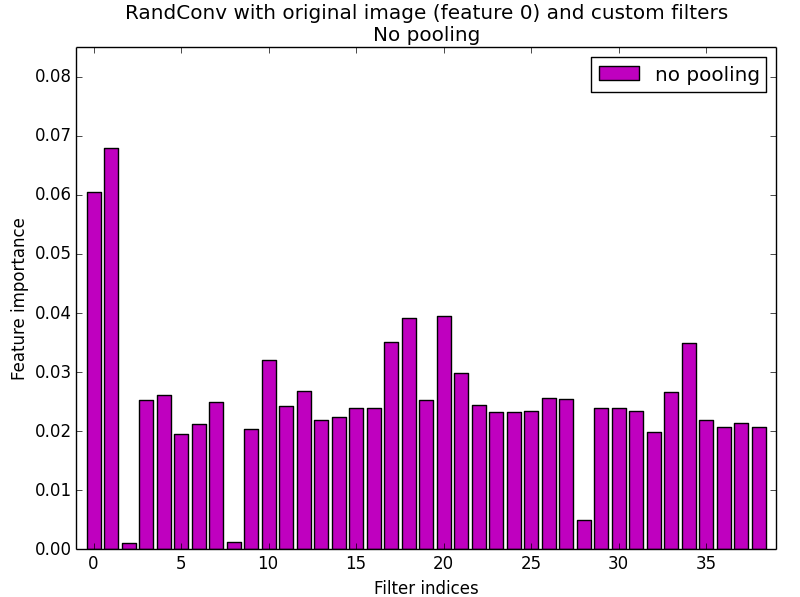
\includegraphics[width=1.\linewidth]{images/FIPoolNo.png}
			\caption{\label{fig:FIPoolNo}}
		\end{subfigure}%
		\begin{subfigure}{.5\textwidth}
			\centering
			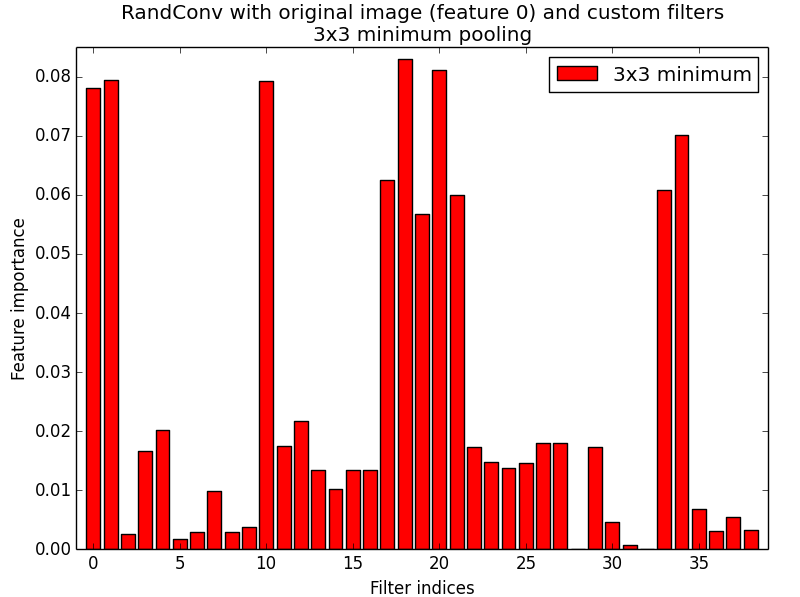
\includegraphics[width=1.\linewidth]{images/FIPoolMin.png}
			\caption{\label{fig:FIPoolMin}}
		\end{subfigure}
		\begin{subfigure}{.5\textwidth}
			\centering
			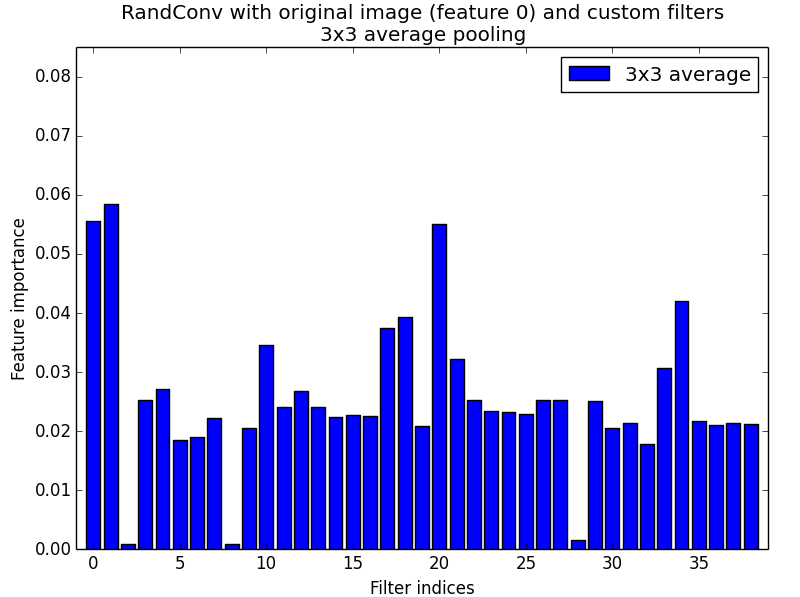
\includegraphics[width=1.\linewidth]{images/FIPoolAvg.png}
			\caption{\label{fig:FIPoolAvg}}
		\end{subfigure}%
		\begin{subfigure}{.5\textwidth}
			\centering
			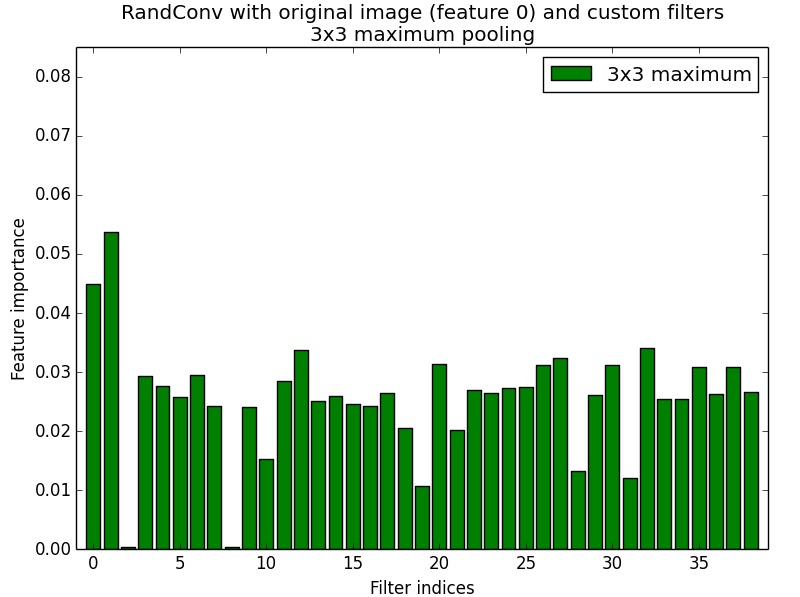
\includegraphics[width=1.\linewidth]{images/FIPoolMax.png}
			\caption{\label{fig:FIPoolMax}}
		\end{subfigure}
		\caption{\label{fig:FIPool}Filter importances with different types of poolings}
	\end{figure}
	
	
	\begin{table}
		\centering
			\begin{tabular}{|c||c|c|c|c|}
			\hline
			Pooling & no pooling & 3x3 minimum & 3x3 average & 3x3 maximum\\
			\hline \hline 
			no pooling & 1 & & &  \\
			\hline
			3x3 minimum & 0.762 & 1 & & \\
			\hline
			3x3 average & 0.954 & 0.826 & 1 & \\
			\hline
			3x3 maximum & 0.723 & 0.226 & 0.661 & 1 \\
			\hline
			\end{tabular}
		\caption{\label{tab:FIPoolCorr}Correlation matrix of the filter importances between the poolings}
	\end{table}
	
	
	\begin{figure}
		\centering
			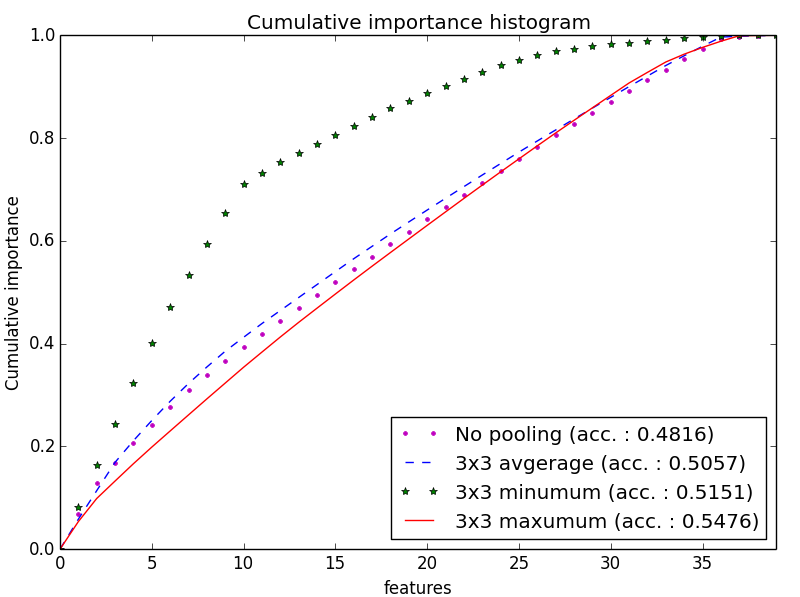
\includegraphics[width=1.0\textwidth]{images/FIPoolCumul.png}
		\caption{\label{fig:FIPoolCumul}Cumulative filter importances with different types of poolings}
	\end{figure}
	
	\par
	The observation of single pooling strategies bode well for their combine application. Yet, it may happen that they shade each other in a co-utilization scenario. In turns out this is a empty threat. The correlation between importances in single pooling strategies and their corresponding importances in multipooling strategies are above 0.96 for all of them (no pooling included). This is visually illustrated by figure \ref{fig:FIPoolNoAvgMinMax}. Each group of four bars belong to the same linear filter. 
	
	\begin{figure}
		\centering
			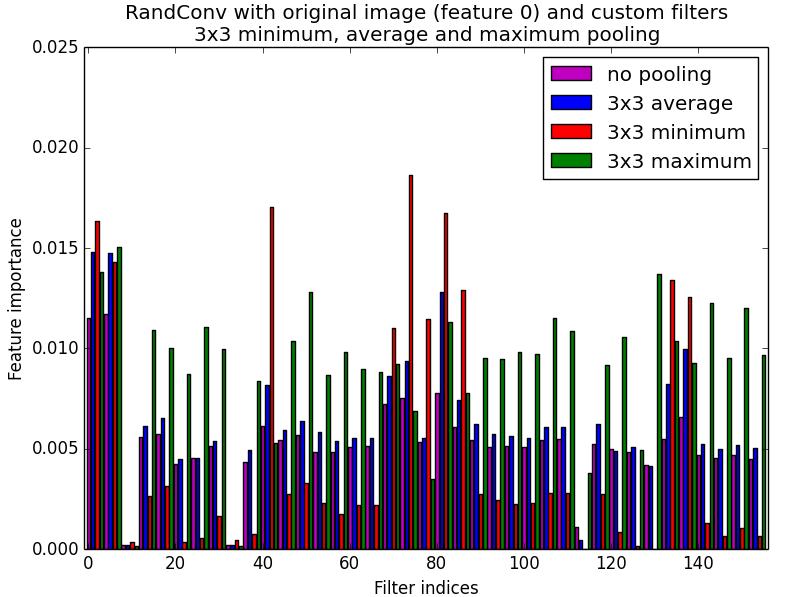
\includegraphics[width=1.0\textwidth]{images/FIPoolNoAvgMinMax.png}
		\caption{\label{fig:FIPoolNoAvgMinMax}Filter importances with several poolings}
	\end{figure}
	
	\par
	Figure \ref{fig:FIPoolScale} displays the filter profile for several poolings only differing by the moving window size. Most filters seems to favor larger windows. This is also the case with the minimum pooling. This (non-)locality preference should be problem dependent.
	
	
	\begin{figure}
		\begin{subfigure}{.5\textwidth}
			\centering
			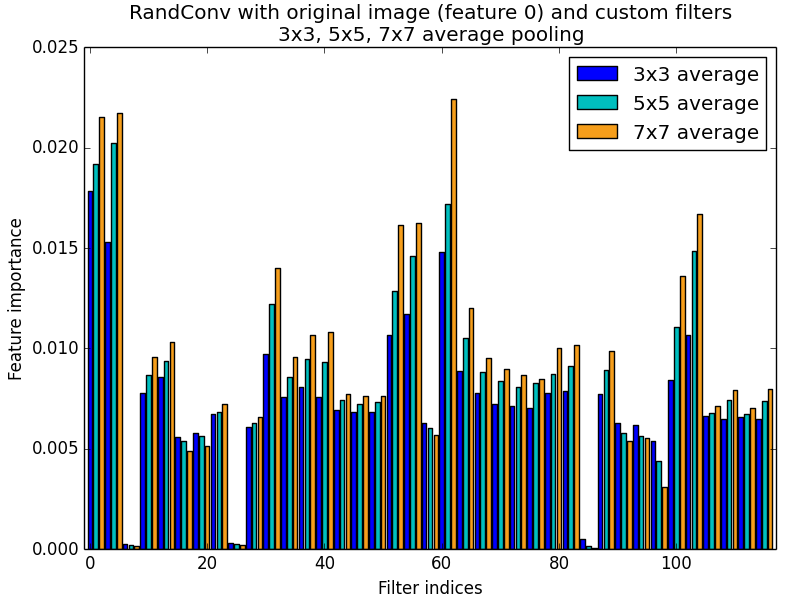
\includegraphics[width=1.\linewidth]{images/FIPoolAvg357.png}
			\caption{\label{fig:FIPoolAvg357}}
		\end{subfigure}%
		\begin{subfigure}{.5\textwidth}
			\centering
			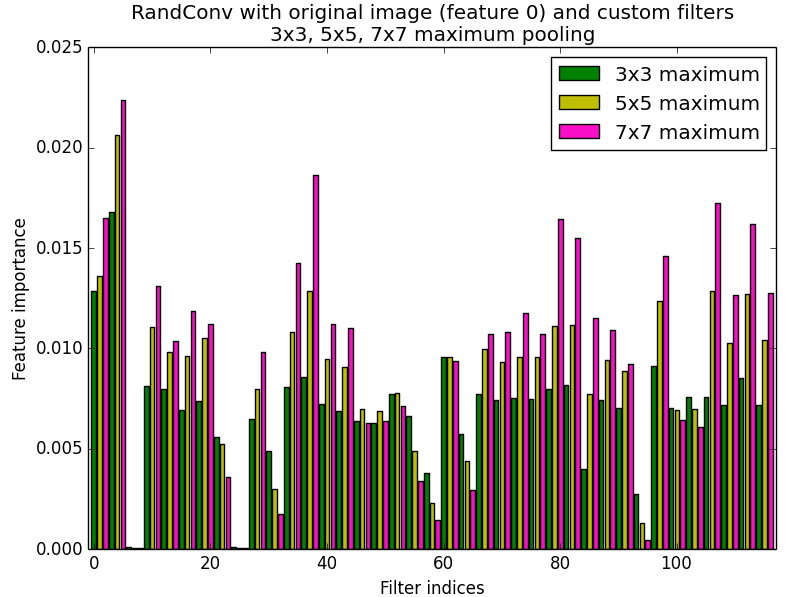
\includegraphics[width=1.\linewidth]{images/FIPoolMax357.png}
			\caption{\label{fig:FIPoolMax357}}
		\end{subfigure}
		\caption{\label{fig:FIPoolScale}Filter importances with several pooling scales}
	\end{figure}
		
	
	\paragraph{}
	Using a more appropriate spatial pooling is what has brought us the best improvement so far. Since poolings do not interfere with each other, an alternative to picking the best one is simply to use several. In doubt, a combination of the minimum and maximum pooling should do. If the best one is known, however, it might be worth investing the extra free memory elsewhere. We basically have two choices : either increasing the number of filters or the number of subwindows. The latter seems more promising from our recent observations.
	
	
	
	\subsection{Influence of the compression}
	In this subsection, we tackle the subvector compression. We ran the RandConv method with the default value except for the feature extraction which uses color compression. The accuracy results for keeping only one or two colors per pixel are respectively 0.5041 and 0.5112. In both cases the confusion matrix seems to be in accordance with those of the previous experiments. Other experiments tends to produce the same kind of results : one color per pixel is usually slightly inferior to two colors per pixel. In any case, the influence of the compression is marginal. This can be exploited to reallocate the freed memory to more interesting parameters.
	\par
	The conclusion on filter importances is as usual : compression does not influence much the filter profiles.
	
	\subsection{\label{subsec:UpperBound}Empirical upper bound on the accuracy}
	We have now had a tour on the influence of the hyper-parameters. Clearly, the most important is the spatial pooling. Then comes the number of trees, the parameters $k$ and the number of subwindows. Sadly, the number of filters and the kind of filter generator play a less important role in the process.
	Based on this observation we can now test an optimal set of parameters. The accuracy we will obtain will be subject to some bias because we did not determine this set of parameters on a independent database. However, the bias should be small. Figure \ref{fig:accFLSsize} about the influence of the database size on accuracy suggests that a database of 40,000 images is representative enough. Furthermore, our observation were either confirming our intuitions or too clear to be dependent on the learning samples only. Finally, we will consider this result for what it is : an upper bound on the accuracy.
	\par
	We chose to use the custom filters with two poolings, a 7x7 minimum and maximum. We impose compression so as to have 2 colors per original pixel. We use the remaining memory to extract 30 subwindows per images. We built 500 trees with a value of $k$ of 500 as well. The final accuracy scores \textbf{0.613}. Of course, this made for a long learning phase (approximately 1 day).
	
	\subsection{Improvements}
	We thought of two improvements for the ET-DIC methods. 
	
	\paragraph{Useful filter selection.}
	The first one was to use the trees to assess the filter usefulness, keep only the best of them and proceeds in an iterative manner to build a stock a ``good'' filters. This selection can be conducted in an unsupervised way and therefore would not suffer from selection bias. The good news brought by the previous section is that we do not need much resources to assess the filter usefulness : the filter profiles are quite stable and can be assessed with totally randomized trees using only 5 subwindows and compression so as to quicken the process and/or allow for more filters. We need to use the same spatial poolings, however. The very bad news is that the filter generation mechanism do not seem to matter as much as we had originally hoped and consequently, the accuracy gain is expected to be small.
	\par
	We ran the following experiment : the default classification with a preprocessing for choosing the 100 best filters out of 1000 random ones. The preprocessing is conducted as proposed by totally randomized trees with only 5 subwindows per images and a compression of 1 color per pixel. 
	Figure \ref{fig:FIOpti} depicts the filter profile. As we can see, we have a very regular profile, much more than what we ever have encountered before. Besides, there is no single useless filter, which is also a first. The accuracy is, however a mild 0.5137 ; not even the best for the default classification.
	Once again, this highlights the fact that the filters do not play a major role in the process.
	
	
	\begin{figure}
		\centering
			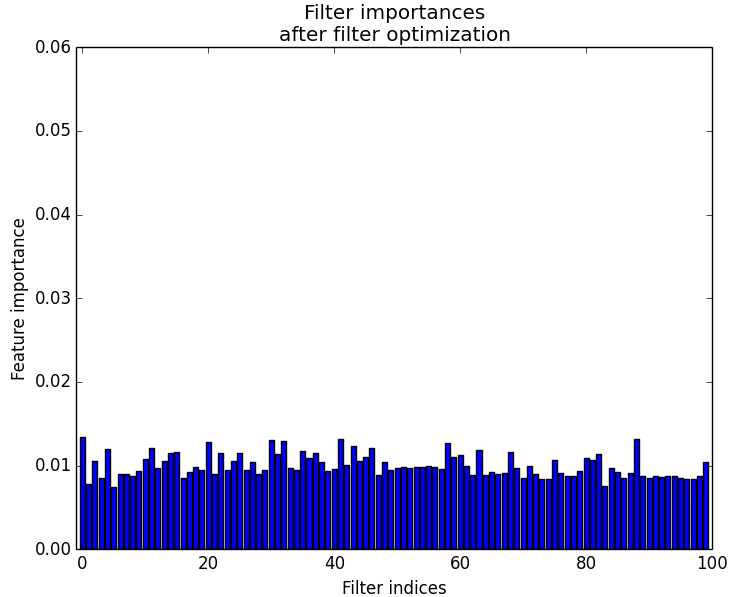
\includegraphics[width=0.7\textwidth]{images/FIOpti.png}
		\caption{\label{fig:FIOpti}Filter importances after optimization of the filter usefulness}
	\end{figure}

	
	
	\paragraph{Global random subspace.}
	%Observation on variability
	The second improvement consists on growing forests independently with different sets of filters, as was mentioned in subsection \ref{sub:TechnicalIssues} about technical issues. The results are aggregated by averaging the class probabilities of a given image. In other words, we vote the class over the several forests.
	Considering the independence of the filters of two different forests and our discussion about the number of filters, we foresee that the main accuracy gain will actually comes from the augmentation of the total number of trees. 
	\par
	We made our experiment using the following filter generators (unmentioned parameters are left to their default values) : 
	\begin{itemize}
		\item Identity-perturbed generator with a real uniform law on $[-1, 1]$ (accuracy : 0.5128)	 % rc_idpert_ru_default.npy
		\item Identity-distance generator with a maximum distance of 10 and a real uniform law (accuracy : 0.4999) %rc_1400617651.npy
		\item Stratified generator with a subdivision in 10 cells and a Gaussian law of 0 mean and 0.021 standard deviation (accuracy : 0.5063) %rc_1400958397.54.npy
	\end{itemize}
	The accuracy was of 0.5241, which is indeed more than the individual accuracies. The total number of trees is of 90. From our previous study on the topic, we can say that the major part of the accuracy gain comes indeed from the increase in the number of trees.
	\par
	We can also add our best result of 0.613 with the custom filters and 500 trees of subsection \ref{subsec:UpperBound}. However, we need to weight appropriately the model predictions, for example by the number of trees. This yields a slight accuracy gain, rising to 0.6137, whereas we would obtain 0.569 without weights. 
	
	
	
	
	
	
	%Fortunately, the default parameters works well --> No optimization bias
	%---------------------------------------------------------------------------%

	
	\section{Feature learning scheme}
	The previous section focused on the ET-DIC pros and cons. We now turn to the ET-FL mode. In this mode, we use totally randomized trees to build a visual dictionary and the actual classification is carried out by a SVM. 
	\paragraph{}
	This mode is less prone to a deep analysis of the hyper-parameters' influences. The parameter $k$ is fixed to 1, and the number of subwindows, the number of trees and the minimum number of samples to split all influence the number of leaves in a well-understood fashion. An increase in the first two will produce an increase of the number of leaves and ultimately of the discriminant power. The number of subwindows will be severely limited by the memory requirement while the number of trees limitation will be the computational time, although to a lesser extent. A good tradeoff must then be found between the number of subwindows and number of filters and spatial poolings. From the information we gathered in the last section, we can say that the number of subwindows will be much more important than the number of filters. The compression can be reused in order to free some extra memory if need be.
	Since we are not averaging the results any longer, we have lost the ability to reduce overfitting and must resort to pruning in order to limit the complexity. Usually, the optimal pruning should be obtained by cross-validation. However, for our database, a good value of $n_{min} = 500$ has already been established (\cite{base}). 
	\paragraph{}
	Before starting, let us remember those two results already established for the ET-FL mode. In traditional Pixit, an accuracy of 0.5007 was achieved with 10 almost fully grown trees and 20 subwindows. As for the use of filters and several poolings, the record was of 0.7431 with 750 totally randomized trees, 20 subwindows and $n_{min} = 500$. 
	
	
	%describe the succession of experiment
	
	
	%\subsection{Accuracy}
	
	\begin{table}
		\centering
			\begin{tabular}{c|c|c}
			\hline
			Test number & Accuracy & Number of leaves\\
			\hline \hline
			1  & 0.6355 & 1,840,523\\
			2 & 0.6349 & 1,845,322 \\
			3 & 0.6381 & 1,815,057 \\
			4 & 0.6352 & 1,840,463 \\
			5 & 0.6436 & 1,828,582 \\
			6 & 0.6392 & 1,805,235 \\
			7 & 0.6406 & 1,833,373\\
			8 & 0.6412 & 1,837,801\\
			\hline
			\hline
			Standard deviation & 0.003 & 13042.06\\
			\hline
			\end{tabular}
		\caption{\label{tab:BagVarTreesOnly}Accuracy and number of leaves variabilities due to the totally randomized trees (ET-FL mode)}
	\end{table}
	
	
\chapter{Conclusion and perspective}
%Confirn on other dataset
%If confirmed --> explore non-linear filter and/or more complex structures
%Going into the frequency space
%less overlap than MW but more than aggreg

 
\bibliographystyle{apalike}
\bibliography{biblio}
  
\end{document}	


